%   DOCUMENT CLASS  %%%%%%%%%%%%%%%%%%%%%%%%%%%%%%%%%%%%%%%%%%%%%%%%%%%%%%%%%%%

%

%   Use the `sfuthesis` class to format your thesis.

%

%   For more information about thesis formatting requirements, go to

%   http://www.lib.sfu.ca/help/publish/thesis or ask a thesis advisor at the

%   SFU Research Commons.

\documentclass{sfuthesis}

%   DOCUMENT METADATA  %%%%%%%%%%%%%%%%%%%%%%%%%%%%%%%%%%%%%%%%%%%%%%%%%%%%%%%%

%

%   Fill in the following information for the title page and declaration of

%   committee page. Please review the Declaration of Committee page

%   instructions on the library's thesis website before completing this page:

%   https://www.lib.sfu.ca/help/publish/thesis/format/declaration-committee

%   Choose the \faculty entry below from the following list:

%

%       - Faculty of Applied Sciences

%       - Faculty of Arts and Social Sciences

%       - Beedie School of Business

%       - Faculty of Communication, Art and Technology

%       - Faculty of Education

%       - Faculty of Environment

%       - Faculty of Health Sciences

%       - Faculty of Science

\title{ChromaGuide: A Multi-Modal Deep Learning Framework for Comprehensive CRISPR-Cas9 Guide RNA Design and Efficacy Prediction}

\thesistype{Proposal}

\author{Amirhossein Daneshpajouh}

\previousdegrees{%

% Add previous degrees here if applicable

% M.Sc., Example University, YYYY\\

% B.Sc., Example University, YYYY

}

\degree{Doctor of Philosophy}

\department{School of Computing Science}

\faculty{Faculty of Applied Sciences}

\copyrightyear{2026}
\semester{Winter 2026}

%   You may include up to six keywords or phrases. Keywords should be separated

%   with semicolons. No punctuation at the end.

\keywords{CRISPR-Cas9; On-Target Prediction; Epigenomic Features; Deep Learning; Transfer Learning; Conformal Prediction; Uncertainty Quantification}

\committee{%

    \chair{TBD}{TBD}

    \member{Dr. Kay C.\ Wiese}{Supervisor \\ Professor, Computing Science}

    \member{Dr. Maxwell W.\ Libbrecht}{Committee Member \\ Associate Professor, Computing Science}

    \member{TBD}{Committee Member \\ TBD}

    \member{TBD}{Examiner \\ TBD}

    \member{TBD}{External Examiner \\ TBD \\ TBD \\ TBD}

}

%   PACKAGES %%%%%%%%%%%%%%%%%%%%%%%%%%%%%%%%%%%%%%%%%%%%%%%%%%%%%%%%%%%%%%%%%%

%

%   Add any packages you need for your thesis here.

%   You don't need to call the following packages, which are already called in

%   the sfuthesis class file:

%

%   - appendix

%   - etoolbox

%   - fontenc

%   - geometry

%   - lmodern

%   - nowidow

%   - setspace

%   - tocloft

%

%   If you call one of the above packages (or one of their dependencies) with

%   options, you may get a "Option clash" LaTeX error. If you get this error,

%   you can fix it by removing your copy of \usepackage and passing the options

%   you need by adding

%

%       \PassOptionsToPackage{<options>}{<package>}

%

%   before \documentclass{sfuthesis}.

%

%   The following packages are a few suggestions you might find useful.

%

%   (1) amsmath and amssymb are essential if you have math in your thesis;

%       they provide useful commands like ``blackboard bold'' symbols and

%       environments for aligning equations.

%   (2) amsthm includes allows you to easily change the style and numbering of

%       theorems. It also provides an environment for proofs.

%   (3) graphicx allows you to add images with \includegraphics{filename}.

%   (4) hyperref turns your citations and cross-references into clickable

%       links, and adds metadata to the compiled PDF.

%   (5) pdfpages lets you import pages of external PDFs using the command

%       \includepdf{filename}. You will need to do this if your research

%       requires an Ethics Statement.

%

\usepackage{amsmath}                            % (1)

\usepackage{amssymb}                            % (1)

\usepackage{amsthm}                             % (2)

\usepackage{graphicx}                           % (3)

\usepackage[pdfborder={0 0 0}]{hyperref}        % (4)

\usepackage{natbib}                             % For bibliography

\usepackage{algorithm}                           % For algorithms

\usepackage{algorithmic}                        % For algorithms

\usepackage{booktabs}                           % For better tables

\usepackage{multirow}                            % For table cells spanning rows

\usepackage{tabularx}                           % For tables with automatic column widths
\newcolumntype{Y}{>{\raggedright\arraybackslash\hyphenpenalty=10000\exhyphenpenalty=10000}X}

\usepackage{tikz}                               % For architecture diagrams
\usetikzlibrary{arrows.meta,positioning,fit,calc}

\usepackage{microtype}                          % Better justification / fewer overfull boxes
\setlength{\emergencystretch}{2em}

% \usepackage{pdfpages}                         % (5)

% ...

% ...

% ...

% ... add your own packages here!

%   OTHER CUSTOMIZATIONS %%%%%%%%%%%%%%%%%%%%%%%%%%%%%%%%%%%%%%%%%%%%%%%%%%%%%%

%

%   Add any packages you need for your thesis here. We've started you off with

%   a few suggestions.

%

%   (1) Use a single word space between sentences. If you disable this, you

%       will have to manually control spacing around abbreviations.

%   (2) Correct the capitalization of "Chapter" and "Section" if you use the

%       \autoref macro from the `hyperref` package.

%   (3) The LaTeX thesis template defaults to one-and-a-half line spacing. If

%       your supervisor prefers double-spacing, you can redefine the

%       \defaultspacing command.

%

\frenchspacing                                    % (1)

\renewcommand*{\chapterautorefname}{Chapter}      % (2)

\renewcommand*{\sectionautorefname}{Section}      % (2)

\renewcommand*{\subsectionautorefname}{Section}   % (2)

% \renewcommand{\defaultspacing}{\doublespacing}  % (3)

% Custom commands for CRISPR terminology

\newcommand{\gRNA}{\text{gRNA}}

\newcommand{\sgRNA}{\text{sgRNA}}

\newcommand{\PAM}{\text{PAM}}

\newcommand{\CasNine}{\text{Cas9}}

\newcommand{\MI}{\text{MI}}

\newcommand{\ECE}{\text{ECE}}

% Theorem environments

\theoremstyle{definition}

\newtheorem{definition}{Definition}[section]

\newtheorem{theorem}{Theorem}[section]

\newtheorem{lemma}{Lemma}[section]

\newtheorem{proposition}{Proposition}[section]

\newtheorem{corollary}{Corollary}[section]

\newtheorem{remark}{Remark}[section]

\newtheorem{hypothesis}{Hypothesis}[chapter]

% ...

% ...

% ...

% ... add your own customizations here!

%   FRONTMATTER  %%%%%%%%%%%%%%%%%%%%%%%%%%%%%%%%%%%%%%%%%%%%%%%%%%%%%%%%%%%%%%

%

%   Title page, committee page, abstract, dedication, acknowledgements, table

%   of contents, etc.

%

%   If your research requires an Ethics Statement, download the pdf from

%   https://www.lib.sfu.ca/help/publish/thesis/regulations#ethics-statement

%   to your thesis folder, then uncomment the appropriate lines below.

\begin{document}

\frontmatter

\maketitle{}

\makecommittee{}

%\addtoToC{Ethics Statement}%

%\includepdf[pagecommand={\thispagestyle{plain}}]{ethics_statement_piii.pdf}%

%\clearpage

\begin{abstract}

Accurate CRISPR-Cas9 genome editing depends on choosing \gRNA{}s that (i) cut efficiently at the intended locus and (ii) avoid unintended cleavage elsewhere in the genome. However, many existing pipelines treat these requirements in isolation---separately scoring on-target efficacy and off-target risk---and often provide only point estimates, limiting decision support under dataset, protocol, and cell-line shift.

This proposal introduces \textbf{ChromaGuide}, a multi-modal deep learning framework for comprehensive \sgRNA\ design built around three coupled components: (1) \textbf{on-target efficacy prediction}, which estimates editing outcomes in the \emph{relevant} chromatin context; (2) \textbf{off-target prediction}, which scores the likelihood and severity of unintended cleavage sites induced by a candidate guide; and (3) \textbf{\sgRNA\ design}, which integrates (1) and (2) to produce an overall design score that explicitly balances predicted on-target efficiency against off-target specificity.

ChromaGuide integrates (a) sequence signals (e.g., ChromeCRISPR-style CNN--GRU and/or foundation-model embeddings), (b) optional \gRNA\ secondary-structure representations, and (c) epigenomic context features (accessibility and histone-mark tracks). It supports calibrated uncertainty for on-target predictions via a bounded-outcome head (e.g., Beta regression) and conformal prediction, and it ranks candidate guides by aggregating multi-site off-target risk with the on-target signal into a single, actionable \sgRNA\ score.

We will evaluate ChromaGuide on DeepHF, CRISPRon, and CRISPR-FMC using leakage-controlled \textbf{gene-held-out} and \textbf{dataset/cell-line-held-out} splits to stress-test generalization. The expected contributions are: (1) a rigorously evaluated multi-modal architecture for on-target efficacy prediction, (2) an off-target prediction module that supports genome-wide unintended-site risk scoring, (3) an integrated \sgRNA\ design score for guide selection that balances efficiency and specificity, and (4) an evaluation protocol that makes failure modes under biological shift visible. If successful, ChromaGuide will enable more reliable, context-aware, and safety-aware \gRNA\ prioritization.

\end{abstract}

% \begin{dedication}
% Optional dedication page
% \end{dedication}

\begin{acknowledgements}

I thank my supervisor, Dr. Kay C. Wiese for his support, guidance and feedback, as well as my supervisory committee and colleagues at Simon Fraser University and the broader computational biology community for enabling this work through open datasets and tools. I am also grateful to my family and friends for their continued support.

\end{acknowledgements}

\addtoToC{Table of Contents}%

\tableofcontents%

\clearpage

\addtoToC{List of Figures}%
\listoffigures%
\clearpage

\addtoToC{List of Tables}%
\listoftables%
\clearpage

%   MAIN MATTER  %%%%%%%%%%%%%%%%%%%%%%%%%%%%%%%%%%%%%%%%%%%%%%%%%%%%%%%%%%%%%%

%

%   Start writing your thesis --- or start \include ing chapters --- here.

%

\mainmatter%

\chapter{Introduction}

\section{Motivation and problem statement}

CRISPR-Cas9 is a programmable RNA-guided nuclease that enables targeted genome editing in eukaryotic cells~\citep{jinek2012,cong2013,hsu2014}. In a standard SpCas9 workflow, a \gRNA{} directs \CasNine\ to a locus adjacent to a \PAM{} (5$'$-NGG-3$'$) on the non-target strand (NTS); recognition occurs via Arg1333 and Arg1335 major-groove contacts with the GG dinucleotide~\citep{jinek2012,anders2014}, while the target-strand complement (5$'$-CCN-3$'$) is not directly read. Downstream double-strand break (DSB) repair then produces an observed editing outcome.

This proposal targets \emph{comprehensive CRISPR-Cas9 guide RNA design and efficacy prediction}: given a candidate \gRNA\ and its genomic target, (i)~estimate on-target cleavage/indel efficiency in the \emph{relevant} cellular context, (ii)~quantify genome-wide off-target risk, and (iii)~produce an integrated design score that balances efficacy and safety. Existing predictors can achieve strong benchmark correlations, but practical deployment remains limited by two recurring issues: (i) models are often sequence-centric and only weakly capture chromatin accessibility/state, and (ii) most models output point estimates without calibrated uncertainty, making it hard to decide when predictions are reliable under dataset/cell-line shift~\citep{horlbeck2016,isaac2016,vovk2005,romano2019,barber2023}.


\section{Proposed approach and thesis overview}

Recent large-scale benchmarking work highlights that strong within-dataset performance does not always translate to reliable generalization across datasets and cell types~\citep{konstantakos2022,chen2022evaluation}.  Our group's prior work established a clear research progression: Daneshpajouh, Fowler, and Wiese~\citep{daneshpajouh2023navitas,daneshpajouh2023comparison} first conducted a systematic comparison of machine learning models for CRISPR/Cas on-target prediction (IEEE CIBCB 2023, Canadian AI 2023), demonstrating that RNNs significantly outperform CNNs and that GC content improves predictions. Building on these findings, ChromeCRISPR (Daneshpajouh, Fowler, and Wiese)~\citep{daneshpajouh2025chromecrispr}---a CNN-RNN hybrid trained on $\sim$60,000 sgRNAs from the DeepHF dataset---achieved state-of-the-art Spearman $\rho=0.876$ (MSE 0.0093), outperforming both DeepHF ($\rho=0.867$) and AttCRISPR ($\rho=0.872$). ChromaGuide extends this validated hybrid architecture by integrating epigenomic context, calibrated uncertainty via conformal prediction, and off-target risk assessment.

Motivated by these findings, we position ChromaGuide against both established sequence-based baselines and recent 2025 deep-learning models, including CRISPR\_HNN~\citep{li2025crisprhnn}, PLM-CRISPR~\citep{hou2025plmcrispr}, CRISPR-FMC~\citep{li2025crisprfmc}, DNABERT-Epi~\citep{kimata2025dnabertepi},  and Graph-CRISPR~\citep{jiang2025graph-crispr}, using the ChromeCRISPR benchmark protocols where applicable~\citep{daneshpajouh2025chromecrispr}.

\textbf{ChromaGuide} is a three-module \sgRNA{} prioritization pipeline:
\begin{enumerate}
    \item \textbf{On-target module:} multi-modal efficacy prediction with uncertainty quantification.
    \item \textbf{Off-target module:} genome-wide off-target site scoring.
    \item \textbf{Design module:} integrated score balancing efficacy and safety.
\end{enumerate}
Operational success is defined by \emph{surpassing current state-of-the-art models} through improved ranking performance on the primary gene-held-out test split (target Spearman $\geq 0.88$ with $\Delta\rho\geq 0.02$ vs.~the ChromeCRISPR baseline when evaluated on the same leakage-controlled split; note that ChromeCRISPR's baseline $\rho=0.876$ was obtained under a different split protocol---see Section~\ref{sec:evaluation} for details) and empirical interval coverage within $\pm 0.02$ of the target level (e.g., 0.90) \emph{under the exchangeability assumption}.

Chapter~\ref{ch:rq} formalizes the research questions, testable hypotheses, operational success criteria, and expected contributions of this work. Chapter~\ref{ch:background} reviews the relevant literature, and Chapter~\ref{ch:methodology} details the proposed methodology.
\chapter{Research Questions and Objectives}

This proposal is organized around three coupled modules: \textbf{(i) on-target efficacy prediction}, \textbf{(ii) off-target risk prediction}, and \textbf{(iii) integrated \sgRNA\ design}. The research questions and hypotheses below are stated so they can be evaluated on leakage-controlled and shift-aware splits.

\section{Research questions and objectives}

\textbf{RQ1 (on-target module):} \emph{How much does adding epigenomic context and multi-modal fusion improve on-target efficacy prediction under realistic generalization constraints (e.g., gene-held-out and dataset/cell-line shift)?}

\textbf{Objective 1 (on-target modeling):} Develop a leakage-evaluated on-target predictor that fuses sequence with epigenomic context (and optional \gRNA{}-structure features) using a fusion mechanism that encourages complementary (non-redundant) representations.

\textbf{RQ2 (off-target module):} \emph{Can an off-target model that uses mismatch/bulge patterns and (when available) local chromatin context produce better guide-level specificity/risk estimates than sequence-only baselines?}

\textbf{Objective 2 (off-target modeling):} Build an off-target module that (i) enumerates plausible unintended sites and (ii) scores each site to yield an aggregated guide-level off-target risk/specificity estimate.

\textbf{RQ3 (integrated \sgRNA\ design):} \emph{Does combining calibrated on-target predictions with aggregated off-target risk improve end-to-end guide ranking for practical \sgRNA\ design compared to optimizing either objective alone?}

\textbf{Objective 3 (end-to-end guide design):} Define and validate an integrated \sgRNA\ design score that jointly ranks candidates by predicted efficiency and specificity, with explicit, tunable trade-offs.

\textbf{Cross-cutting objective (uncertainty and shift):} Provide distribution-free prediction intervals for on-target outcomes via split conformal prediction \emph{under the exchangeability assumption} (including weighted variants for dataset/cell-line shift, which rely on (estimated) importance weights / likelihood ratios)~\citep{vovk2005,romano2019,barber2023}, and evaluate transfer learning under low-resource and shifted settings~\citep{pan2010,liao2025primenet,mathis2024pridict2}.

\section{Testable hypotheses}

\begin{hypothesis}[On-target generalization gain]
\label{hyp:h1}
On leakage-controlled gene-held-out splits, adding epigenomic context and multi-modal fusion improves on-target predictive performance (e.g., Spearman correlation) over a strong sequence-only baseline.
\end{hypothesis}

\textbf{Operationalization:} On a pre-registered, leakage-controlled gene-held-out test split (Split~A), ChromaGuide improves Spearman correlation over the chosen baseline by at least $\Delta\rho = 0.004$ (e.g., $0.876\to 0.880$) while maintaining conformal prediction-interval coverage within $\pm 0.02$ of the target level (e.g., 0.90). (ChromeCRISPR's reported $\rho=0.876$ was obtained under a random 85/15 split; we will re-evaluate the baseline under Split~A for like-for-like comparison.)

\begin{hypothesis}[Off-target risk estimation gain]
\label{hyp:h2}
Conditioned on the same candidate guides, incorporating chromatin context (when available) improves per-site off-target scoring and the resulting aggregated guide-level off-target risk/specificity estimate compared to sequence-only scoring.
\end{hypothesis}

\textbf{Operationalization:} On an off-target benchmark with measured unintended sites, the chromatin-aware model improves a ranking metric (e.g., AUROC/AUPRC for site classification or NDCG/Top-$k$ recall for site ranking) over the sequence-only baseline, and this improvement persists under cell-line-held-out evaluation when epigenomic tracks are available.

\begin{hypothesis}[Integrated design improves guide ranking]
\label{hyp:h3}
A joint \sgRNA\ design score that combines calibrated on-target predictions with aggregated off-target risk yields better guide ranking than optimizing on-target alone or off-target alone.
\end{hypothesis}

\textbf{Operationalization:} When ranking candidate guides per target (gene/region), the integrated score improves Top-$k$ selection quality (e.g., probability that at least one of the top-$k$ guides is high-efficacy and low-risk) relative to (i) on-target-only ranking and (ii) off-target-only ranking, under the same evaluation splits.

\section{Expected contributions}

\begin{itemize}
\item \textbf{Multi-modal on-target efficacy prediction:} a leakage-evaluated model that fuses sequence, optional \gRNA\ structure, and ENCODE-style epigenomic context features to predict on-target editing outcomes, with optional calibrated uncertainty.
\item \textbf{Chromatin-aware off-target risk prediction:} an off-target module that enumerates plausible unintended sites and scores them (mismatch/bulge patterns and, when available, local chromatin context) to produce aggregated guide-level specificity/risk estimates.
\item \textbf{End-to-end \sgRNA\ design score:} a practical ranking score that explicitly balances predicted on-target efficiency against aggregated off-target risk to support complete guide RNA design.
\item \textbf{Evaluation protocol for biological shift:} a set of leakage-controlled gene-held-out and dataset/cell-line-held-out splits (and stress tests) that make generalization and uncertainty failure modes visible.
\end{itemize}

\section{Chapter roadmap}

Chapter~1 introduces CRISPR-Cas9 guide design and motivates the need for context-aware, uncertainty-aware prediction. Chapter~2 (this chapter) states the research questions, hypotheses, and expected contributions. Chapter~3 reviews relevant literature (CRISPR biology, epigenomics, existing predictors, uncertainty, and transfer learning). Chapter~4 describes the proposed methodology for the on-target, off-target, and integrated design modules. Chapter~5 presents the evaluation plan and expected results, emphasizing leakage-controlled gene-held-out tests and cross-domain (dataset/cell-line) stress tests. Chapter~6 provides the project timeline, and Chapter~7 discusses broader impacts.

\chapter{Background and Literature Review}\label{chap:litreview}
\sloppy

This chapter summarizes the minimum background needed to motivate \textbf{ChromaGuide}: (i) what drives CRISPR-Cas9 on-target efficacy, (ii) how existing predictors model it, and (iii) the key gaps (context and calibrated uncertainty) addressed in this proposal.

\section{CRISPR-Cas9 on-target efficacy: essential biology}

\begin{figure}[htbp]
\centering
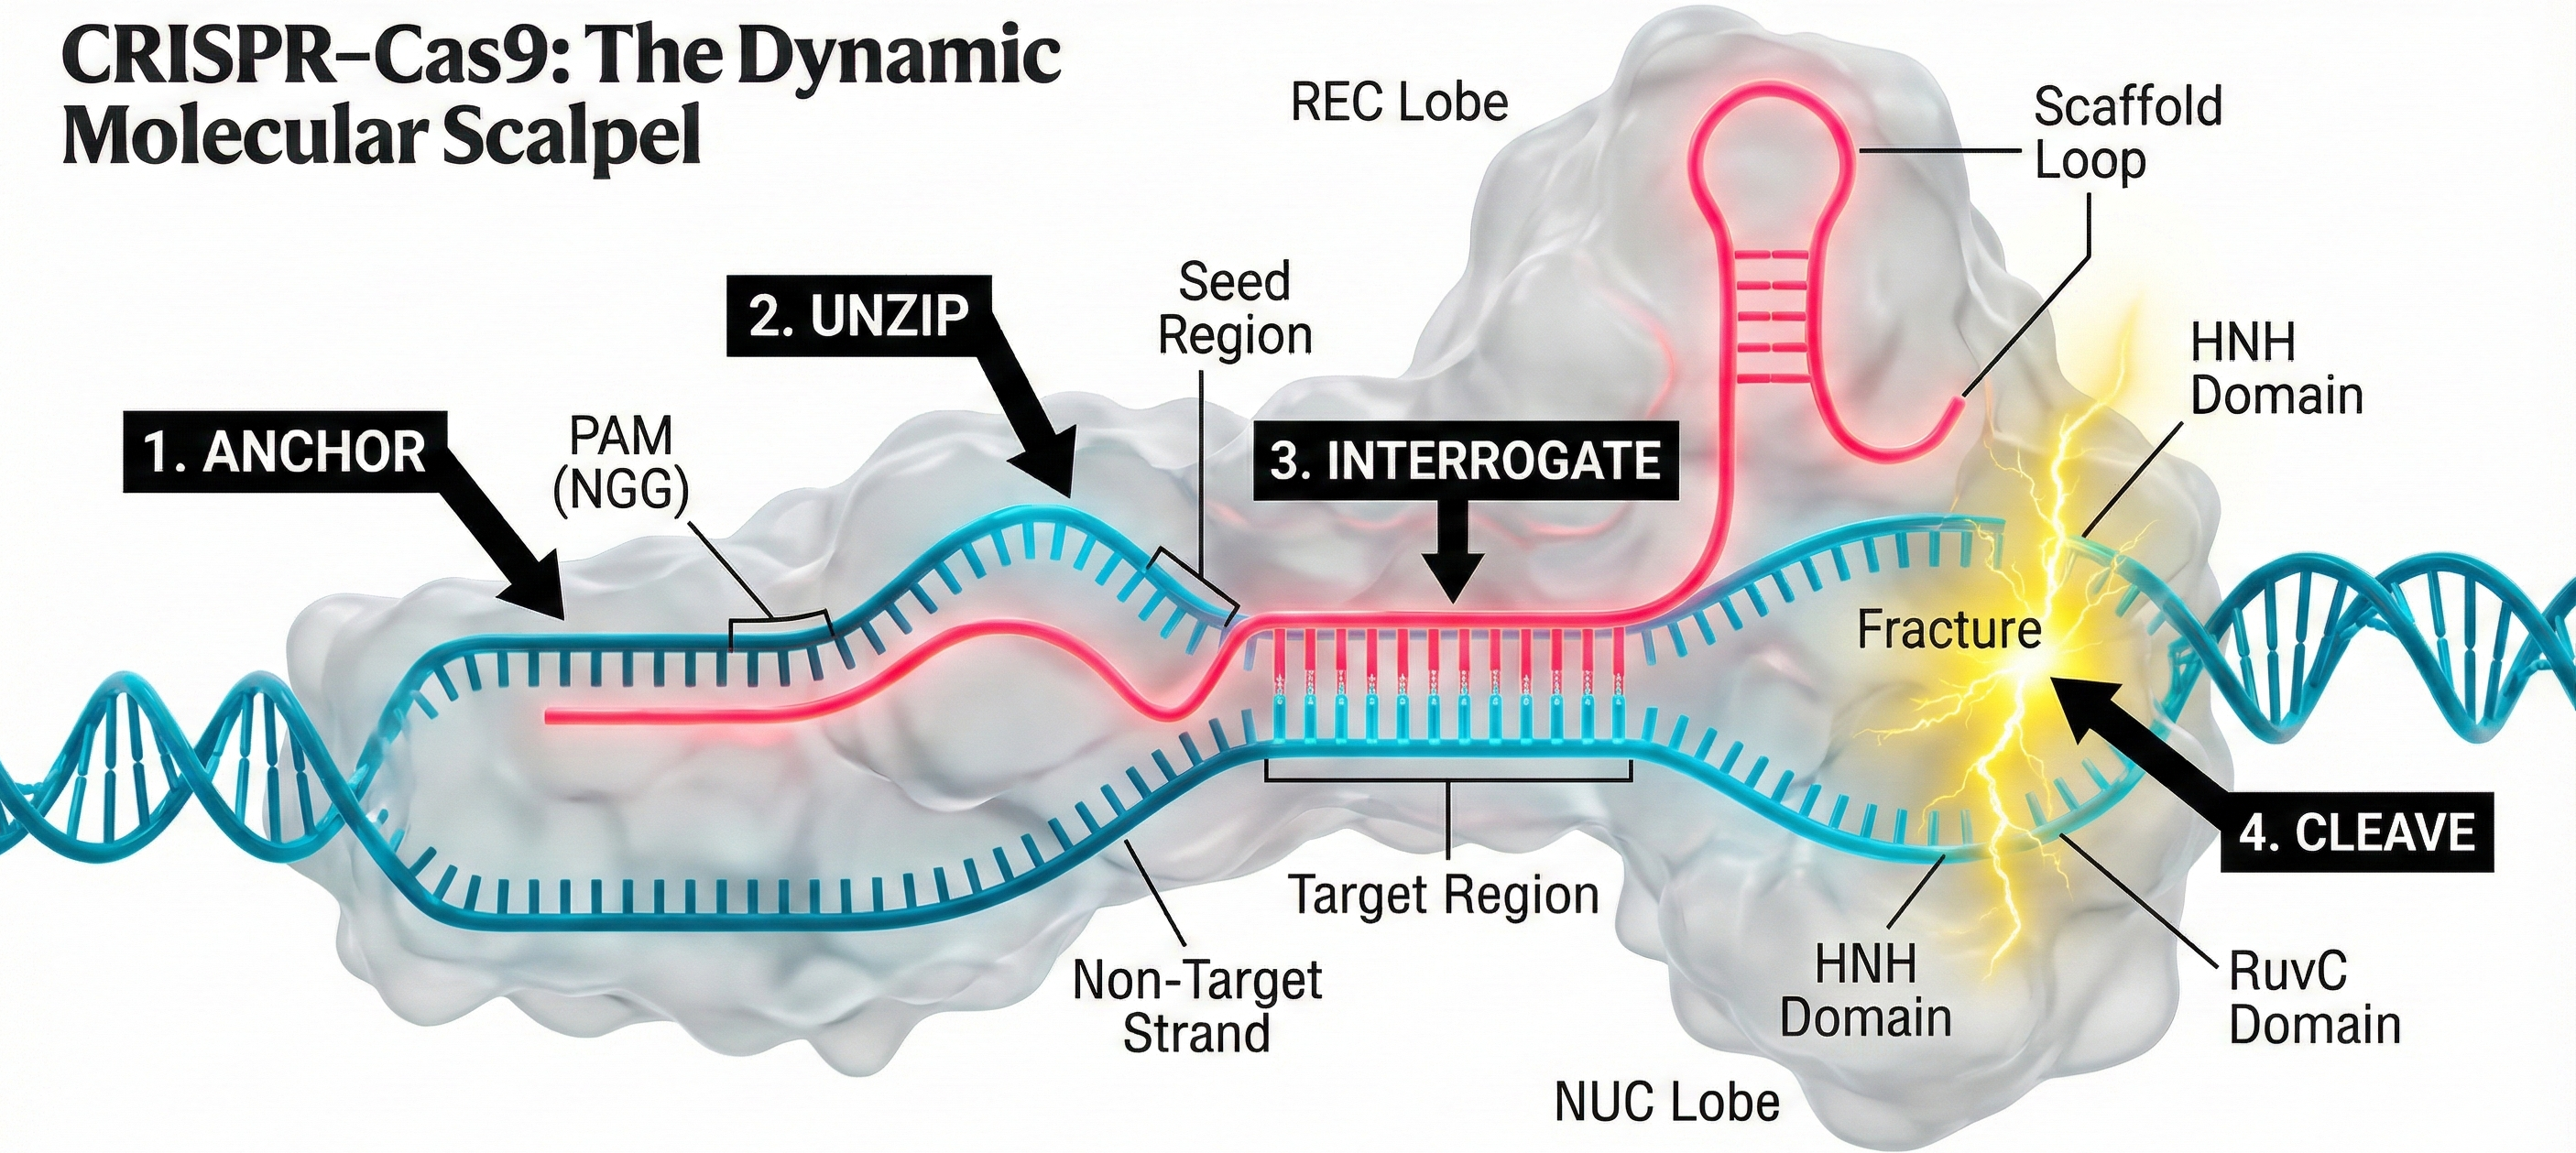
\includegraphics[width=0.9\textwidth]{Figs/CRISPR-Cas9.png}
\caption{CRISPR-Cas9 mechanism showing the four-step process: (A) PAM recognition and anchoring, (B) DNA unwinding, (C) seed region interrogation, and (D) target cleavage.}
\label{fig:crispr-mechanism}
\end{figure}

SpCas9 editing requires a \(\sim 20\)-nt protospacer and a nearby \PAM{} (typically NGG), followed by \CasNine\ binding and cleavage~\citep{jinek2012,hsu2014}. Observed efficacy varies with:
\begin{itemize}
\item \textbf{Sequence effects} (motifs/composition such as GC content).
\item \textbf{\gRNA\ structure/thermodynamics} that can influence guide availability.
\item \textbf{Chromatin accessibility/state} that modulates Cas9 access (e.g., nucleosome occupancy and accessibility)~\citep{horlbeck2016,isaac2016}.
\end{itemize}

\section{On-target predictors: what is typically modeled}

Most on-target predictors map a sequence representation (one-hot, engineered features, or pretrained embeddings) through a learned backbone (CNN/RNN/attention) to output an efficacy score. Representative baselines include DeepHF~\citep{wang2019}, DeepSpCas9~\citep{kim2019deepspcas9}, and ChromeCRISPR~\citep{daneshpajouh2025chromecrispr}. Context-aware models incorporate chromatin accessibility or related epigenomic signals when available, such as CRISPRon~\citep{xiang2021}.

\paragraph{Very recent (2025) on-target models (verified for this thesis scope).}
To keep this proposal concise while reflecting the latest literature, we highlight five 2025 models that motivate the ChromaGuide design space:
\begin{itemize}
\item \textbf{CRISPR\_\allowbreak HNN} (Li et al., 2025): a hybrid MSC +\allowbreak multi-head self-attention (MHSA) +\allowbreak BiGRU model for on-target activity prediction~\citep{li2025crisprhnn}.
\item \textbf{PLM-CRISPR} (Hou et al., 2025): cross-variant prediction that represents Cas9 variants using ESM2 protein language model embeddings~\citep{hou2025plmcrispr}.
\item \textbf{CRISPR-FMC} (Li et al., 2025): a dual-branch architecture for on-target prediction that fuses one-hot sequence features with pretrained RNA embeddings via cross-branch interactions~\citep{li2025crisprfmc}.
\item \textbf{Graph-CRISPR} (Jiang et al., 2025): a graph neural network model that integrates sequence and \sgRNA\ secondary structure features for on-target efficiency prediction~\citep{jiang2025graph-crispr}.
\item \textbf{ChromeCRISPR} (Daneshpajouh et al., 2025): a CNN+RNN (CNN--GRU) hybrid baseline for on-target prediction, emphasizing strong sequence modeling with lightweight auxiliary features (e.g., GC content)~\citep{daneshpajouh2025chromecrispr}.
\end{itemize}

\paragraph{Why protocol choice matters.}
Reported headline metrics remain sensitive to dataset choice and leakage/split design; realistic evaluation therefore requires gene-held-out and cross-domain (dataset/cell-line) stress tests.

% Table omitted for concision (models discussed in text).

\section{Off-target effects and prediction methods}

Off-target activity arises when a \gRNA\ partially matches additional genomic loci that are adjacent to a compatible \PAM{} and permissive to Cas9 binding and cleavage. Key determinants include (i) mismatch number and position (with the PAM-proximal ``seed'' typically less tolerant), (ii) mismatch type and local sequence context, (iii) DNA/RNA bulges, and (iv) chromatin accessibility and other epigenomic factors that can modulate cleavage probability at both intended and unintended loci.

\paragraph{Experimental profiling of off-targets.}
Genome-wide assays such as GUIDE-seq provide empirical off-target site lists and approximate relative activities, and are commonly used to benchmark computational predictors and guide model training/evaluation~\citep{tsai2015guideseq}.

\paragraph{Four families of computational methods.}
Off-target prediction methods can be grouped into:
\begin{enumerate}
\item \textbf{Alignment-based:} enumerate candidate off-target loci by genome-wide approximate matching under PAM and mismatch/bulge constraints (e.g., Cas-OFFinder)~\citep{bae2014casoffinder}.
\item \textbf{Formula-based:} compute mismatch-position-weighted scores (e.g., MIT score, CFD score) and aggregate them into guide-level specificity estimates (often used in pipelines such as CRISPOR)~\citep{doench2016,haeussler2016}.
\item \textbf{Energy-based:} approximate Cas9--\gRNA--DNA binding/cleavage energetics to score the likelihood of cleavage.
\item \textbf{Deep learning / foundation models:} learn site-level cleavage probabilities directly from \sgRNA\--target pairs, optionally integrating epigenomic context (e.g., DeepCRISPR, CCLMoff, DNABERT-Epi)~\citep{chuai2018,du2025cclmoff,kimata2025dnabertepi}.
\end{enumerate}

\paragraph{Recent SOTA: CCLMoff (Du et al., 2025).}
Du et al. introduced \textbf{CCLMoff}, a transformer-based off-target predictor that incorporates a pretrained RNA language model and reports AUROC $=0.996$ in a cross-dataset evaluation setting (train on CIRCLE-seq, test on GUIDE-seq), outperforming a range of prior deep learning baselines~\citep{du2025cclmoff}.

\paragraph{Epigenomics-aware foundation model: DNABERT-Epi (Kimata \& Satou, 2025).}
Kimata and Satou introduced \textbf{DNABERT-Epi}, which fine-tunes a DNABERT foundation model and integrates epigenetic features (H3K4me3, H3K27ac, and ATAC-seq). They benchmark against five baselines across seven off-target datasets and report competitive or superior performance, highlighting the value of combining sequence pretraining with local chromatin context for off-target risk prediction~\citep{kimata2025dnabertepi}.

\section{\sgRNA\ design principles and tools}

Practical \sgRNA\ design aims to select guides with high on-target activity while controlling off-target risk, under hard constraints such as PAM availability and experiment-specific requirements (e.g., U6 promoter compatibility). This is commonly operationalized as (i) generating candidate guides at a locus, (ii) predicting on-target efficacy, (iii) screening/penalizing off-targets, and (iv) selecting a final guide under an explicit efficiency--specificity trade-off.

\paragraph{Taxonomy of on-target predictors.}
On-target efficiency models can be grouped into:
\begin{itemize}
\item \textbf{Conventional ML:} feature-engineered models such as Azimuth/Rule Set 2~\citep{doench2016}.
\item \textbf{Deep learning / pretrained models:} sequence models that learn representations directly from data, sometimes augmented with thermodynamic/structural/epigenomic signals or pretrained embeddings (e.g., CRISPRon, DeepHF, DeepSpCas9, CRISPR\_HNN, CRISPR-FMC, Graph-CRISPR, PLM-CRISPR)~\citep{xiang2021,wang2019,kim2019deepspcas9,li2025crisprhnn,li2025crisprfmc,jiang2025graph-crispr,hou2025plmcrispr}.
\end{itemize}

\begin{sloppypar}
\paragraph{Anchor models and benchmarks.}
Classic deep learning baselines remain widely used: CRISPRon~\citep{xiang2021}, DeepHF~\citep{wang2019}, and DeepSpCas9~\citep{kim2019deepspcas9}. A benchmark and ensemble study by Chen and Wang (Bioinformatics 2022) compared 17 published scoring algorithms across 16 datasets totaling $>90{,}000$ gRNAs and identifies CRISPRon, DeepSpCas9, and DeepHF as top-performing individual predictors, with ensemble approaches (e.g., sgDesigner and TSAM) also ranking strongly~\citep{chen2022ensemble}.
\end{sloppypar}

\paragraph{Very recent 2025 trends.}
Recent SOTA work emphasizes (i) hybrid local+global architectures with dynamic feature weighting (CRISPR\_HNN)~\citep{li2025crisprhnn}, (ii) pretrained embeddings and cross-modal fusion (CRISPR-FMC; Graph-CRISPR)~\citep{li2025crisprfmc,jiang2025graph-crispr}, and (iii) cross-variant generalization by integrating Cas9 variant representations from protein language models (PLM-CRISPR)~\citep{hou2025plmcrispr}.

\paragraph{Design tools.}
End-to-end design tools implement candidate enumeration and integrate on-target and off-target scoring (e.g., CRISPOR, CHOPCHOP), often with practical filters and batch scoring capabilities~\citep{haeussler2016,labun2016chopchop}.

\chapter{Proposed Methodology}
\label{ch:methodology}

\section{Overview}

\textbf{Goal.} ChromaGuide is a three-component framework for \sgRNA\ design that couples (i) \textbf{on-target efficacy prediction}, (ii) \textbf{off-target prediction} (unintended cleavage-site risk), and (iii) an \textbf{integrated \sgRNA\ design score} that balances predicted efficiency and specificity.

\textbf{Task 1 (on-target).} Given a guide/target pair in a cellular context, predict on-target efficacy $y\in[0,1]$ and (optionally) output a prediction interval with target coverage $1-\alpha$.

\textbf{Task 2 (off-target).} Given a candidate \sgRNA\ and a reference genome, identify plausible unintended cleavage sites and score their cleavage likelihood/severity, producing an aggregated off-target risk summary.

\textbf{Task 3 (design score).} Combine the calibrated on-target signal with the aggregated off-target risk to produce an overall \sgRNA\ design score for ranking candidate guides.

\textbf{Inputs.}
\begin{itemize}
\item \textbf{Sequence} $x_s$: \sgRNA\ protospacer+\PAM{} and target-site sequence context.
\item \textbf{Epigenomics} $x_e$: accessibility/histone-mark tracks summarized in a fixed window around (on-target and, when available, off-target) cut sites.
\item \textbf{Genome index/search} $\mathcal{G}$: reference genome data structure used to enumerate candidate off-target loci.
\end{itemize}

\textbf{Core modules (baseline design; alternatives are evaluated via ablation).}
\begin{itemize}
\item On-target encoders: sequence encoder $z_s=g_s(x_s)$ and epigenomic encoder $z_e=g_e(x_e)$.
\item On-target fusion: $z=f([z_s;z_e])$ (baseline concatenation; optional attention/gating; optional non-redundancy regularizer).
\item On-target head: bounded-outcome head producing $(\mu,\phi)$ (baseline Beta regression) and conformal prediction for calibrated intervals~\citep{vovk2005,romano2019,barber2023}.
\item Off-target candidate generation: enumerate candidate loci using genome-wide approximate matching (PAM-constrained) with a bounded mismatch/bulge policy.
\item Off-target scoring network: score each candidate off-target site using sequence mismatch features and optional local context features (sequence, chromatin accessibility when available).
\item Design-score aggregator: combine the on-target prediction with an aggregated off-target risk to produce a single \sgRNA\ design score.
\end{itemize}


\begin{figure}[htbp]
\centering
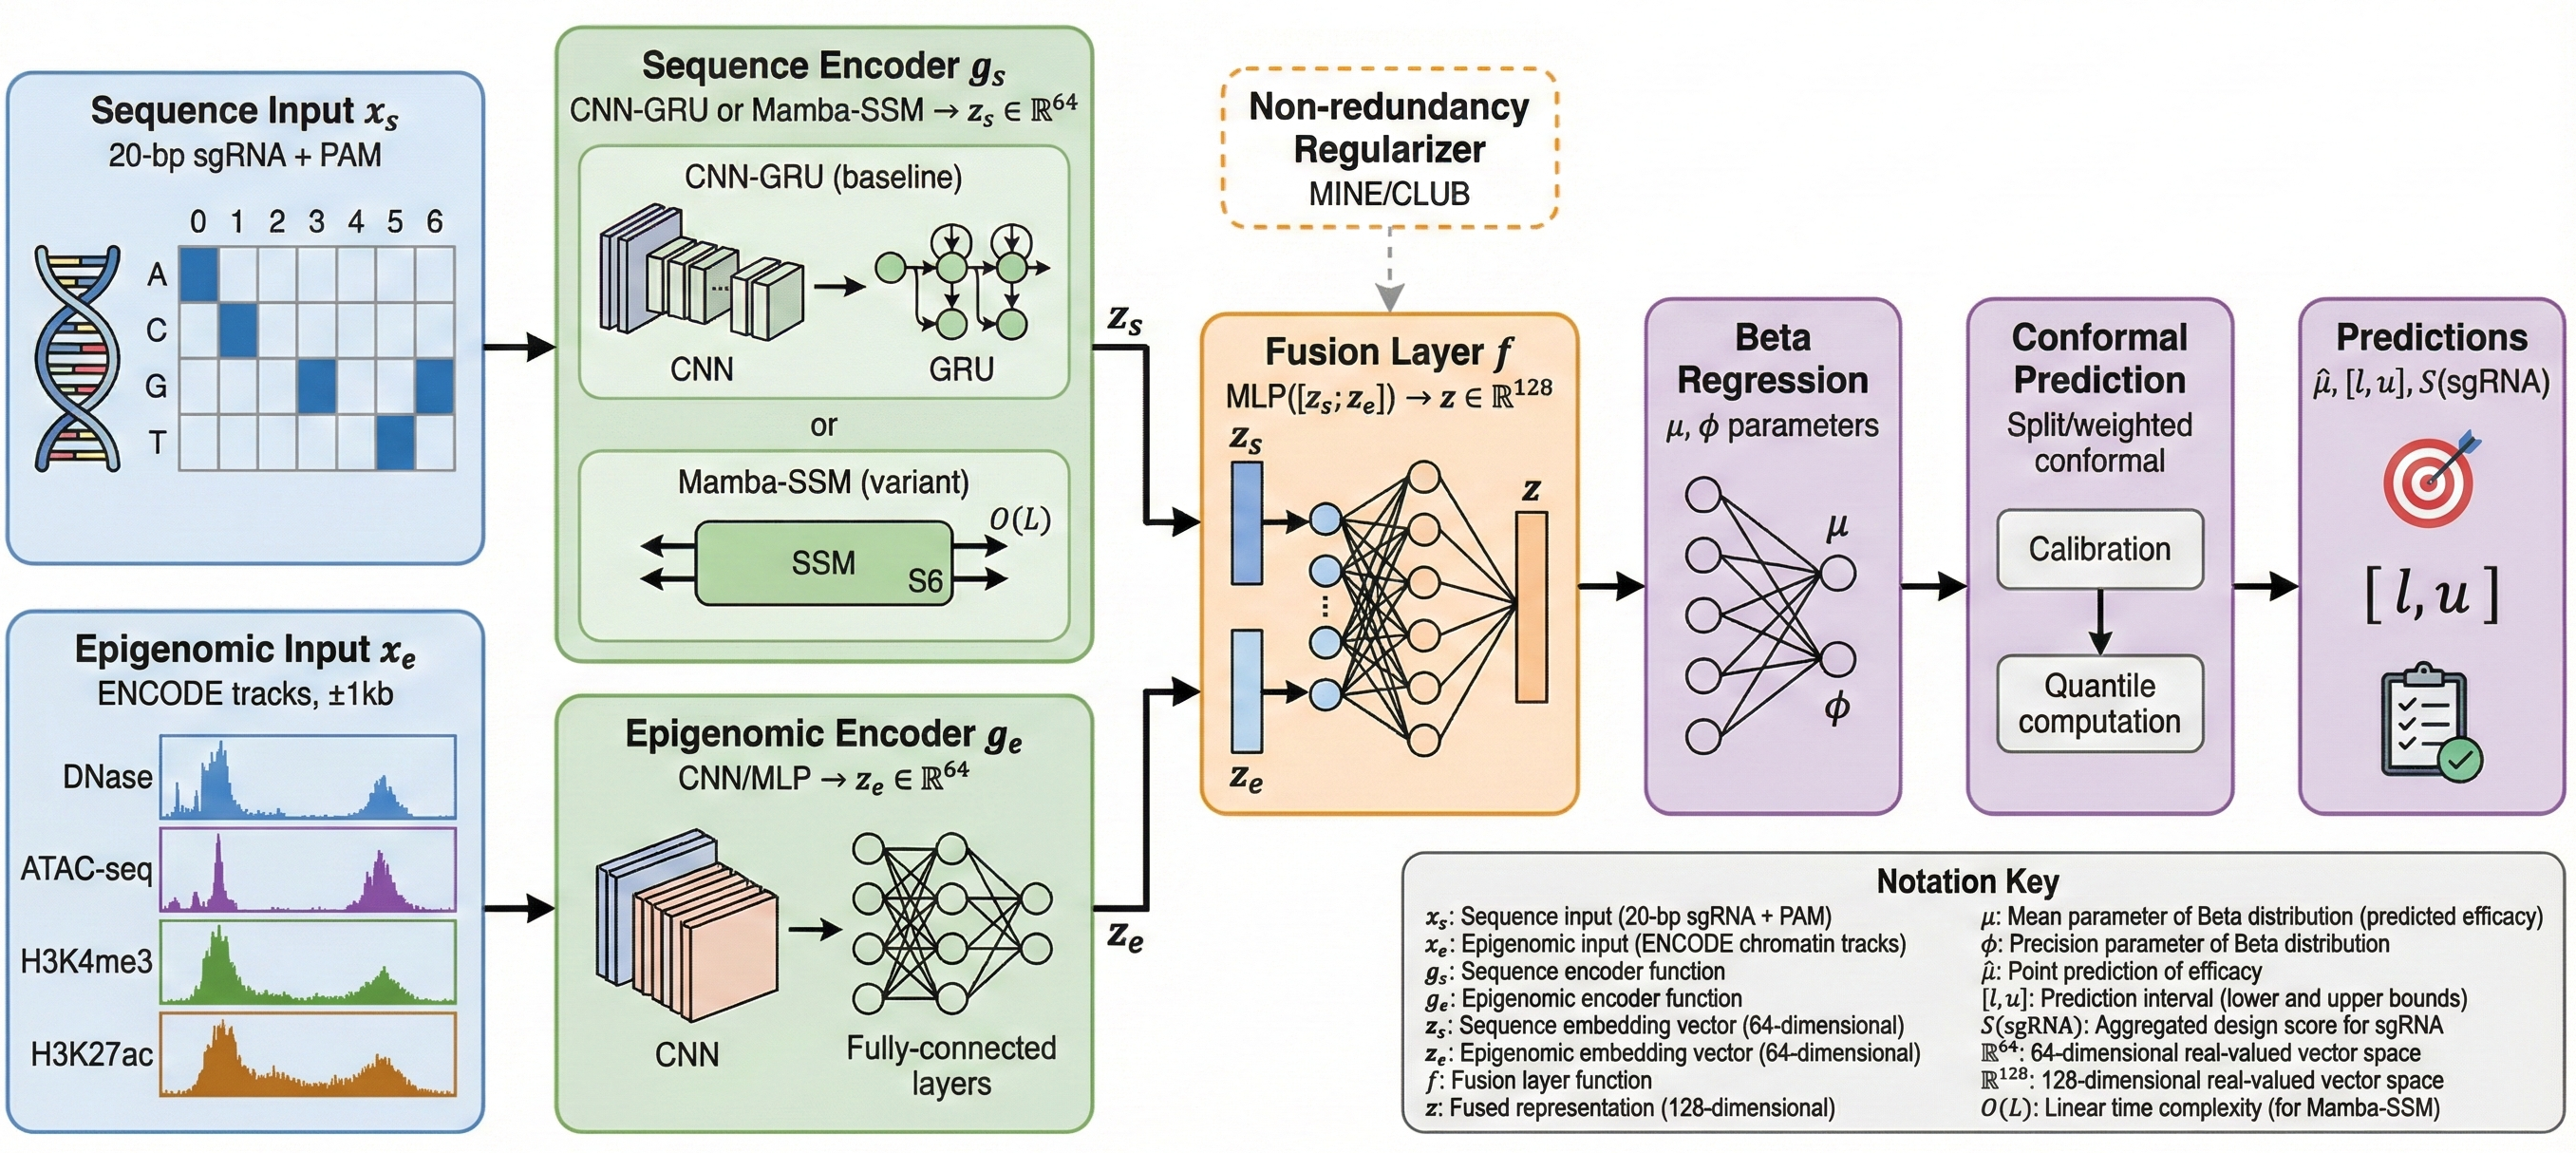
\includegraphics[width=\textwidth]{Figs/ChromaGuide.png}
\caption{ChromaGuide architecture overview. The framework fuses sequence representations with epigenomic context features through a fusion layer. The sequence encoder supports two architectures: (1) a CNN-GRU baseline, or (2) a Mamba-based state-space model (SSM) variant with bi-directional processing and $O(L)$ linear complexity. Inputs: $\mathbf{x}_s$ (one-hot encoded 23-nt sgRNA+PAM sequence (20-nt protospacer + 3-nt PAM)), $\mathbf{x}_e$ (epigenomic tracks). Encoders: $g_s$ (sequence encoder) and $g_e$ (epigenomic encoder) produce embeddings $\mathbf{z}_s, \mathbf{z}_e \in \mathbb{R}^{64}$. Fusion layer $f$ produces $\mathbf{z} \in \mathbb{R}^{128}$. Beta regression outputs parameters $\mu$ (mean) and $\phi$ (precision). Conformal prediction generates calibrated intervals. Final outputs: point prediction $\hat{\mu}$, prediction interval $[l, u]$, and design score $S(\text{sgRNA})$. Optional non-redundancy regularizer (MINE/CLUB) encourages complementary representations.}
\label{fig:proposed-architecture}
\end{figure}

\section{Model architecture}


\subsection{\texorpdfstring{Sequence encoder $g_s$}{Sequence encoder gs}}

\begin{sloppypar}
Baseline: ChromeCRISPR-style CNN--GRU on 23-nt sgRNA+\PAM{} (CNN kernels 3/5/7 $\to$ BiGRU hidden 128 $\to$ pooled $z_s\in\mathbb{R}^{64}$). As contemporary alternatives, we will evaluate (i) hybrid architectures with dynamic feature weighting as in CRISPR\_HNN~\citep{li2025crisprhnn} and (ii) pretrained language-model embeddings for cross-variant generalization as in PLM-CRISPR~\citep{hou2025plmcrispr}. Transformer-based DNA/RNA embeddings (e.g., DNABERT-2, Nucleotide Transformer) and state-space model (SSM) backbones (e.g., Mamba) are included as planned architectural ablations to determine whether modern pretrained representations improve upon the CNN-GRU baseline inherited from ChromeCRISPR.
\end{sloppypar}

\textbf{Structured ablation protocol.} Table~\ref{tab:ablation-backbone} specifies the backbone comparison design. All ablations share identical downstream components (same fusion layer, same prediction head, same training budget of 100 epochs on a single A100 GPU), varying only the sequence encoder. Selection criteria: the backbone yielding the highest validation Spearman $\rho$ on Split~A (gene-held-out) is adopted as the final encoder; ties are broken by parameter count (fewer preferred).

\begin{table}[h]
\centering
\small
\caption{Structured backbone ablation design. All conditions use identical fusion, head, and training configuration.}
\label{tab:ablation-backbone}
\begin{tabular}{llccc}
\hline
\textbf{Backbone} & \textbf{Type} & \textbf{Params (M)} & \textbf{Pretrained} & \textbf{$d_{\text{out}}$} \\
\hline
CNN-GRU (baseline) & Convolutional+Recurrent & $\sim$2 & No & 64 \\
DNABERT-2 & Transformer (6-mer) & $\sim$117 & Yes & 64 \\
Nucleotide Transformer & Transformer (6-mer) & $\sim$500 & Yes & 64 \\
Caduceus-PS & Mamba SSM (bi-dir) & $\sim$7 & Yes & 64 \\
Evo (7B, frozen+adapter) & StripedHyena & $\sim$14 (adapter) & Yes & 64 \\
\hline
\end{tabular}
\end{table}

\begin{sloppypar}
Beyond Transformers, we will explore \textbf{state-space models (SSMs)} as an alternative sequence encoder architecture. Mamba~\cite{gu2023mamba} introduced selective state spaces with input-dependent gating, achieving linear-time complexity $O(L)$ while maintaining expressive long-range modeling. For genomic applications, Caduceus~\cite{schiff2024caduceus} extended Mamba with bi-directional processing and reverse-complement (RC) equivariance, demonstrating superior performance on long-range DNA sequence tasks at the ICML 2024 conference. The Evo model~\cite{nguyen2024evo} scaled long-context genome modeling to 131kb using the StripedHyena architecture (a hybrid attention + long convolution design), demonstrating that long-range encoders can capture regulatory elements across large genomic loci. Recent work has shown that pre-trained DNA language models can substantially improve CRISPR on-target efficacy prediction when fine-tuned on guide-specific datasets~\citep{li2025crisprfmc,hou2025plmcrispr}, motivating the use of foundation model encoders in our sequence branch. Separately, DNABERT-Epi~\citep{kimata2025dnabertepi} demonstrated that integrating epigenetic features with pre-trained DNA language models significantly improves CRISPR \emph{off-target} prediction; we leverage a similar epigenomic integration strategy in our off-target module (Section~\ref{sec:offtarget}). We will benchmark a Mamba-based variant of our sequence encoder against the CNN-GRU baseline, evaluating whether SSMs provide computational efficiency gains without sacrificing predictive accuracy for sgRNA design tasks.
\end{sloppypar}


\subsection{\texorpdfstring{Epigenomic encoder $g_e$}{Epigenomic encoder ge}}

For each assay (e.g., DNase/ATAC, H3K4me3, H3K27ac), extract a window (default $\pm 1$ kb) around the cut site, bin into fixed-length features, apply log1p and training-only standardization, and map through an MLP to $z_e\in\mathbb{R}^{64}$. Additional tracks/encoders (e.g., 1D CNNs over binned tracks) are evaluated in ablation as alternative architectures for epigenomic encoding if the baseline MLP proves insufficient. 

\textbf{ENCODE cell-line mapping.} The DeepHF benchmark uses three cell lines: HEK293T, HCT116, and HeLa. We source matched epigenomic tracks from the ENCODE portal~\citep{encode2020} as follows: (i)~\textbf{HEK293T}: DNase-seq (ENCSR000ENM), H3K4me3 ChIP-seq (ENCSR000DTU), and H3K27ac ChIP-seq (ENCSR000FCJ); (ii)~\textbf{HCT116}: DNase-seq (ENCSR000ENO), H3K4me3 ChIP-seq (ENCSR000DWN), and ATAC-seq (ENCSR000EOJ); (iii)~\textbf{HeLa}: DNase-seq (ENCSR000ENP), H3K4me3 ChIP-seq (ENCSR000DWE), and H3K27ac ChIP-seq (ENCSR000FCG). All signal tracks are aligned to hg38 and processed as fold-change-over-control bigWig files. For cell lines where a specific assay is unavailable, we set the corresponding input channel to zero and include an assay-availability indicator feature. This explicit mapping ensures that ChromaGuide's multi-modal premise is grounded in concrete, reproducible, and empirically justified data sources. These three tracks were selected because they capture complementary aspects of the chromatin environment relevant to \CasNine\ access: DNase-seq/ATAC-seq directly measures physical DNA accessibility at the cut site, H3K4me3 marks active promoter regions where guide targeting is most frequent, and H3K27ac identifies active enhancers and regulatory elements where chromatin state modulates cleavage efficiency. Together they provide broad coverage of ENCODE-profiled cell types while remaining tractable for multi-modal training; repressive marks (e.g., H3K9me3, H3K27me3) are excluded from the default set but may be explored in ablation studies.

\subsection{\texorpdfstring{Fusion $f$ and optional non-redundancy regularizer}{Fusion f and optional non-redundancy regularizer}}

Our proposed default fusion strategy is \textbf{gated attention fusion}, selected based on preliminary experiments; the final choice will be determined by systematic ablation comparison and may be revised if alternative strategies (e.g., cross-attention or mixture-of-experts) demonstrate superior performance: $z=\mathrm{GatedAttn}([z_s;z_e])\in\mathbb{R}^{128}$, where a learned gating vector $g=\sigma(W_g[z_s;z_e]+b_g)$ modulates the element-wise contribution of each modality before a final projection layer. This mechanism was selected because (i) it allows the model to dynamically weight sequence vs.\ epigenomic features per sample, which is critical when chromatin accessibility varies across cell lines, and (ii) gated fusion has demonstrated superior performance over simple concatenation in related multi-modal genomics tasks. As planned ablations, we additionally evaluate concatenation+MLP, cross-attention, and mixture-of-experts fusion to validate this design choice (see Table~\ref{tab:ablation-backbone}). Hyperparameter optimization will be conducted via \textbf{Bayesian optimization} using the Optuna framework~\citep{akiba2019optuna} with a Tree-structured Parzen Estimator (TPE) sampler over 50 trials, optimizing validation Spearman $\rho$ on Split~A. The search space includes learning rate ($[10^{-5}, 10^{-2}]$ log-uniform), dropout rate ($[0.05, 0.4]$), hidden dimension ($\{64, 128, 256\}$), batch size ($\{32, 64, 128\}$), and fusion gate initialization bias ($[-1, 1]$). Early stopping with patience of 15 epochs prevents overfitting during each trial.

We optionally encourage complementary representations with an information-theoretic objective:
\begin{equation}\label{eq:fusion}
f^* = \arg\max_{f \in \mathcal{F}} \left[ I(f(X_s, X_e); Y) - \lambda \cdot I(X_s; X_e | Y) \right],
\end{equation}
implemented with neural MI estimators (e.g., MINE/CLUB)~\citep{belghazi2018,cheng2020} and treated strictly as an ablation.

\subsection{Prediction head (Beta regression)}

Predict a Beta mean and precision:
\begin{equation}
\mu = \sigma(W_\mu z + b_\mu),\qquad \phi = \exp(W_\phi z + b_\phi).
\end{equation}
Negative log-likelihood:
\begin{equation}\label{eq:beta_loss}
\begin{split}
L = -\sum_{i=1}^N \Big[ &\log \Gamma(\phi_i) - \log \Gamma(\mu_i \phi_i) - \log \Gamma((1-\mu_i)\phi_i) \\
&\quad + (\mu_i \phi_i - 1) \log y_i + ((1-\mu_i)\phi_i - 1) \log(1-y_i) \Big].
\end{split}
\end{equation}
We clip $y$ to $(\varepsilon,1-\varepsilon)$ when needed; Beta regression is standard for continuous outcomes in $(0,1)$~\citep{ferrari2004beta}.

\section{Uncertainty quantification via conformal prediction}

Split conformal prediction yields distribution-free prediction intervals \emph{under the exchangeability assumption}~\citep{vovk2005,romano2019}. With a Beta head, define
$$
\hat{\sigma}=\sqrt{\frac{\hat{\mu}(1-\hat{\mu})}{1+\hat{\phi}}},\qquad s=\frac{|y-\hat{\mu}|}{\hat{\sigma}+\varepsilon}.
$$
On calibration data compute $\hat{\eta}=\mathrm{Quantile}_{1-\alpha}(\{s_i\})$ and output
$$
C(x)=\left[\hat{\mu}(x)-\hat{\eta}\,\hat{\sigma}(x),\;\hat{\mu}(x)+\hat{\eta}\,\hat{\sigma}(x)\right]\cap[0,1].
$$
For dataset/cell-line shift (Splits B/C), use weighted conformal calibration, which relies on (estimated) importance weights / likelihood ratios and may degrade under severe shift~\citep{barber2023}.

\section{Off-target prediction  module}

\textbf{Exchangeability under gene-held-out evaluation.} For Split~A (gene-held-out), we acknowledge that strict exchangeability may not hold because guides targeting different genes inhabit distinct genomic contexts with varying GC content and chromatin environments. We address this through two complementary strategies. First, we empirically verify approximate exchangeability by comparing the marginal feature distributions (sequence composition, predicted secondary structure energy, and epigenomic signal statistics) between calibration and test gene groups using two-sample Kolmogorov--Smirnov tests; if the null hypothesis of identical distributions is not rejected at $\alpha=0.05$ for all features, we report standard conformal coverage. Second, as a robustness check, we apply weighted conformal prediction to Split~A using gene-level importance weights estimated via logistic regression on a binary gene-group indicator, following the framework of \citet{barber2023}. We report both the standard and weighted coverage for Split~A, clearly distinguishing between the finite-sample guarantee (valid only under exchangeability) and the empirical coverage (always reported). If weighted and standard coverage diverge by more than 2 percentage points, we flag the gene-held-out split as exhibiting non-trivial covariate shift and interpret the conformal intervals as approximate rather than distribution-free. \textbf{Marginal vs.\ conditional coverage.} We note that standard conformal prediction provides \emph{marginal} coverage---i.e., averaged over all test points---rather than \emph{conditional} coverage for any specific input $x$. The gap between marginal and conditional coverage can be significant when the model's uncertainty varies across the input space (e.g., high-GC vs.\ low-GC guides, open vs.\ closed chromatin regions). To partially bridge this gap, we stratify the empirical coverage analysis by (i) GC-content quartile, (ii) chromatin accessibility quartile, and (iii) gene functional category, reporting per-stratum coverage alongside the global marginal rate. If per-stratum coverage falls below $(1-\alpha) - 0.05$ for any subgroup, we apply the group-conditional conformal procedure of~\citet{barber2023} to recalibrate intervals within that stratum, accepting the corresponding reduction in statistical efficiency.
\label{sec:offtarget}

\subsection{Candidate unintended-site identification}

Given a candidate \sgRNA{}, ChromaGuide first enumerates plausible off-target loci by scanning the reference genome for PAM-adjacent protospacer matches under an explicit mismatch/bulge policy. Concretely, we (i) require a valid PAM (e.g., NGG for SpCas9; optionally extend to alternative PAMs when modeling SpCas9 variants), (ii) allow up to $m$ mismatches with position-dependent weighting (penalizing mismatches less in distal regions than in the seed), and (iii) optionally allow a small number of DNA/RNA bulges, depending on computational feasibility.

This stage outputs a set of candidate off-target sites $\{o_j\}$, each with its genomic coordinates and an alignment summary (mismatch positions/types and bulge indicators). To keep the proposal implementable and the document within a $\sim$30-page scope, we treat the genome search as a modular component (e.g., using an indexed approximate matching routine) and focus the research contribution on learning to score the resulting candidate set.

\subsection{Off-target scoring}

For each candidate site $o_j$, we compute a feature vector that includes (a) aligned guide--DNA sequence pairs / mismatch pattern encodings, (b) local sequence context around the cut site, and (c) optional cell-context features (e.g., accessibility) when tracks are available for the corresponding locus. This is motivated by recent off-target models that integrate epigenetic tracks with sequence representations (e.g., DNABERT-Epi)~\citep{kimata2025dnabertepi}. A neural scoring function outputs a per-site risk $r_j\in[0,1]$ that is intended to correlate with cleavage likelihood and/or editing readouts in available off-target datasets.

\textbf{Training data.} The off-target scoring model is trained on experimentally validated off-target sites from GUIDE-seq~\citep{tsai2015guideseq} and CIRCLE-seq~\citep{tsai2017circleseq} datasets, which together provide $\sim$200k labeled guide--off-target pairs across multiple cell lines. Positive labels indicate biochemically or cellularly validated cleavage events; negatives are PAM-adjacent genomic sites with no detected cleavage above background. We apply the same gene-level deduplication strategy described in \S\ref{sec:evaluation} to avoid train/test overlap on homologous loci.

\textbf{Scoring architecture.} The per-site scoring function $f_{\text{OT}}$ is a three-layer convolutional neural network (CNN) with 1D convolutions over the aligned guide--target pair (kernel sizes 3, 5, 7 to capture local and extended mismatch context), followed by global average pooling and two fully connected layers ($d=128 \to 64 \to 1$) with a sigmoid output producing $r_j \in [0,1]$. When cell-specific chromatin features are available, they are concatenated after the pooling layer. The model is trained with binary cross-entropy loss and class-weight balancing to handle the strong negative-class imbalance ($\sim$50:1 in GUIDE-seq).

To summarize genome-wide risk for a guide, we aggregate across sites using a soft-max/Noisy-OR style pooling function, for example
$$
R(\sgRNA)=1-\prod_j (1-r_j) \quad \text{or} \quad R(\sgRNA)=\sum_j w_j r_j,
$$
where weights $w_j$ can encode distance-to-gene, exonic overlap, or other application-driven severity terms. As an additional baseline family for off-target scoring, we will consider language-model-based off-target predictors such as CCLMoff~\citep{du2025cclmoff}.

\textbf{Saturation mitigation.} The Noisy-OR form saturates toward $R\to 1$ when many candidate sites have non-negligible $r_j$, making all guides appear equally risky. To prevent this, we apply two safeguards: (i)~only the top-$k$ highest-scoring off-target sites are included in the aggregation (default $k=20$), pruning low-confidence hits that inflate the product; and (ii)~a temperature parameter $\tau$ scales each per-site probability as $r_j^{1/\tau}$ before aggregation, allowing the model to interpolate between a hard-max ($\tau\to 0$) and the standard Noisy-OR ($\tau=1$). The choice of $k$ and $\tau$ will be selected via the validation split to maximize rank correlation with observed guide-level specificity.

\section{Integrated \sgRNA\ design score}

ChromaGuide ranks candidate guides using an integrated design score that explicitly trades off efficiency and specificity. This is aligned with recent \sgRNA\ prediction/design models that explicitly integrate richer guide representations (e.g., sequence + secondary structure via graph neural networks in Graph-CRISPR)~\citep{jiang2025graph-crispr}. Let $\hat{\mu}(\sgRNA)$ denote the predicted on-target efficacy (mean of the bounded head) and let $R(\sgRNA)$ denote aggregated off-target risk. A simple, interpretable baseline is
$$
S(\sgRNA)=\hat{\mu}(\sgRNA)-\lambda\,R(\sgRNA),
$$
with $\lambda>0$ controlling the efficiency--specificity trade-off; alternative monotone combinations (e.g., $S=\hat{\mu}\cdot(1-R)$) are treated as ablations.

When uncertainty estimates are available, we will also evaluate risk-aware ranking rules that down-weight uncertain high-efficacy predictions (e.g., replacing $\hat{\mu}$ with a lower confidence bound).


\textbf{Formal design score aggregator.} For the complete ChromaGuide design score, we define $S(\text{sgRNA})$ as a weighted combination of on-target efficacy, off-target safety, and uncertainty:
$$
S(\text{sgRNA}) = w_e \cdot \hat{\mu}(\text{sgRNA}) - w_r \cdot R(\text{sgRNA}) - w_u \cdot \sigma_{\text{CI}}(\text{sgRNA}),
$$
where $\hat{\mu}(\text{sgRNA})$ is the predicted on-target efficacy (mean of the Beta regression head), $R(\text{sgRNA}) = \sum_j r_j$ is the aggregated off-target risk score summed over all candidate off-target sites, $\sigma_{\text{CI}}(\text{sgRNA})$ is the width of the conformal prediction interval (capturing epistemic uncertainty), and $w_e, w_r, w_u > 0$ are user-adjustable weights with defaults $w_e=1.0$, $w_r=0.5$, $w_u=0.2$. All component scores are min-max normalized to $[0,1]$ before aggregation. This formulation allows experimentalists to tune the efficiency--safety trade-off for their application: therapeutic contexts may increase $w_r$ to prioritize specificity, while screening applications may decrease it to maximize hit rate.
\section{\sgRNA\ design tool / interface module}\label{sec:design-interface}

To satisfy the third ChromaGuide module requirement (a user-facing design capability rather than only predictive models), we will implement an interface that accepts either (i) a genomic target region (e.g., gene name / coordinates) or (ii) a user-provided DNA sequence, enumerates candidate protospacers with valid PAMs, and returns a ranked list with supporting diagnostics. This is conceptually similar to widely used \sgRNA\ design tools (e.g., CRISPOR and CHOPCHOP) but adds uncertainty-aware on-target estimates and an explicit chromatin-aware risk model~\citep{haeussler2016,labun2016chopchop}.

\paragraph{Inputs.} User-selected genome build; target coordinates or sequence; nuclease/PAM (SpCas9 NGG by default); optional cell type / epigenomic context (select ENCODE track set or upload summarized tracks).

\paragraph{Outputs.} For each candidate guide: predicted on-target efficacy (with interval), aggregated off-target risk $R(\sgRNA)$, integrated design score $S(\sgRNA)$, and a short explanation panel (top contributing sequence positions and key epigenomic bins). The tool will also export results as a CSV/TSV report to support downstream wet-lab planning.

\paragraph{Workflow (high level).}
\begin{enumerate}
\item Enumerate candidate guides in the target region under PAM and basic filters (e.g., homopolymer and GC constraints).
\item Compute on-target predictions with epigenomic integration when context is available; otherwise fall back to sequence-only mode.
\item Enumerate and score candidate off-target loci genome-wide, aggregate $R(\sgRNA)$, and compute $S(\sgRNA)$.
\item Rank guides and present the top-$m$ candidates with uncertainty-aware summaries.
\end{enumerate}

\section{Practical considerations (brief)}

\textbf{Missing epigenomics (modality dropout training).} Train with modality dropout by masking $x_e$ (or assay subsets) with probability $p$ and adding a missingness indicator, so the model degrades to sequence-only behavior when tracks are absent.

\textbf{Optional extensions.} RNA-FM embeddings, a lightweight \gRNA\ structure branch, and transfer initialization (PRIDICT/PrimeNet, ) are optional and always ablated.

\textbf{Implementation defaults.} Adam/AdamW~\citep{kingma2015,loshchilov2019}, early stopping on calibration, and tuning restricted to train+calibration splits.

\textbf{Computational budget.} We estimate the total compute requirement at approximately 800--1,200 A100 GPU-hours across all experiments. The baseline CNN-GRU model ($\sim$2M parameters) trains in $\sim$4 hours per fold on a single A100-80GB. The largest backbone ablation (Nucleotide Transformer, $\sim$500M parameters with frozen trunk and trainable adapter) requires $\sim$12 hours per fold. With 5 backbone variants $\times$ 3 splits $\times$ 3 cell lines, plus the epigenomic ablation (5 conditions $\times$ 3 splits), hyperparameter sweeps (50 Optuna trials per configuration), and the off-target module training, the total budget is feasible within a single-GPU allocation over approximately 3--4 months. We have secured access to 4$\times$ NVIDIA A100-80GB GPUs through SFU's Fir cluster allocation (RAC 2026).


\textbf{Complete training objective.} The on-target module is trained by minimizing a composite loss:
$$
\mathcal{L} = \mathcal{L}_{\text{MSE}} + \lambda_{\text{cal}}\mathcal{L}_{\text{cal}} + \lambda_{\text{NR}}\mathcal{L}_{\text{NR}},
$$
where $\mathcal{L}_{\text{MSE}} = \frac{1}{N}\sum_{i=1}^{N}(\hat{y}_i - y_i)^2$ is the primary regression loss on clipped Spearman-transformed efficacy scores, $\mathcal{L}_{\text{cal}}$ is a calibration-aware penalty (expected calibration error on held-out validation bins), and $\mathcal{L}_{\text{NR}} = -\hat{I}(\mathbf{z}_s; \mathbf{z}_e)$ is the mutual-information-based non-redundancy regularizer operating on the \emph{learned} sequence and epigenomic representations $\mathbf{z}_s \in \mathbb{R}^{64}$ and $\mathbf{z}_e \in \mathbb{R}^{64}$ (not the raw inputs), estimated via the MINE lower bound~\citep{belghazi2018}. We set $\lambda_{\text{cal}}=0.1$ and $\lambda_{\text{NR}}=0.01$ as defaults, with both treated as tunable hyperparameters in ablation. Training uses AdamW~\citep{kingma2015,loshchilov2019} with initial learning rate $\eta=5\times10^{-4}$, weight decay $0.01$, linear warm-up for 5 epochs followed by cosine annealing to $\eta_{\min}=10^{-6}$, batch size 256, and gradient clipping at max-norm 1.0. Early stopping monitors validation Spearman $\rho$ with patience 15 epochs. The off-target module uses binary cross-entropy with class-weight balancing (positive weight $\approx$20:1 reflecting the strong class imbalance in GUIDE-seq data) and the same optimizer configuration except initial $\eta=10^{-3}$ and batch size 512.
\textbf{Methodological flexibility.} The architectural choices, hyperparameter configurations, and specific tools described throughout this chapter represent our current best design based on the existing literature and preliminary analysis. As is standard in PhD research, these decisions remain subject to revision as empirical results accumulate. Specifically: (1)~the fusion strategy (gated attention) may be replaced if ablation experiments reveal that cross-attention, mixture-of-experts, or another mechanism yields consistently superior performance; (2)~the sequence encoder backbone (CNN-GRU baseline with foundation model ablations) may shift toward a different architecture if emerging models or transfer learning approaches prove more effective for CRISPR guide prediction; (3)~the epigenomic track selection and window sizes may be adjusted based on feature importance analysis and data availability for additional cell lines; (4)~the statistical testing framework (Holm-Bonferroni/Benjamini-Hochberg) may be supplemented or refined based on the observed data distributions; and (5)~the hyperparameter optimization strategy may be adapted if the search landscape warrants different approaches. All such modifications will be documented and justified in the final thesis. The evaluation protocol---gene-held-out splits, conformal prediction for uncertainty quantification, and the core research questions---constitutes the stable methodological backbone that will persist regardless of component-level changes.

\section{Evaluation plan (summary)}\label{sec:evaluation}

\textbf{Datasets.} Primary (initial): DeepHF~\citep{wang2019}. Stress tests (initial): CRISPRon~\citep{xiang2021} and the CRISPR-FMC compiled dataset~\citep{li2025crisprfmc}. \textbf{Cell-line validation strategy:} Primary model development and hyperparameter tuning use HEK293T data from DeepHF (the largest single-cell-line CRISPR efficacy dataset). Cross-cell-line generalization is validated on HCT116 (colorectal carcinoma) and HeLa (cervical carcinoma) subsets, which represent distinct chromatin landscapes and transcriptional programs. For each validation cell line, we source matched epigenomic tracks from ENCODE (see Section~\ref{sec:epigenomic-encoder}) and evaluate whether models trained on HEK293T maintain predictive performance ($\Delta\rho \leq 0.05$ degradation) when applied to held-out cell lines. If cross-cell-line degradation exceeds this threshold, we apply cell-line-specific fine-tuning with 10\% of the target cell-line data as a practical transfer learning strategy.

\textbf{Splits (leakage-controlled).}
\begin{itemize}
\item \textbf{Split A (primary):} gene-held-out split on DeepHF with train/cal/test by gene.
\item \textbf{Split B (stress test):} dataset-held-out evaluation (e.g., leave-one-dataset-out across CRISPR-FMC compiled-dataset constituents).
\item \textbf{Split C (stress test):} cell-line-held-out evaluation (train excluding one cell line; test on held-out line).
\end{itemize}

\begin{figure}[htbp]
\centering
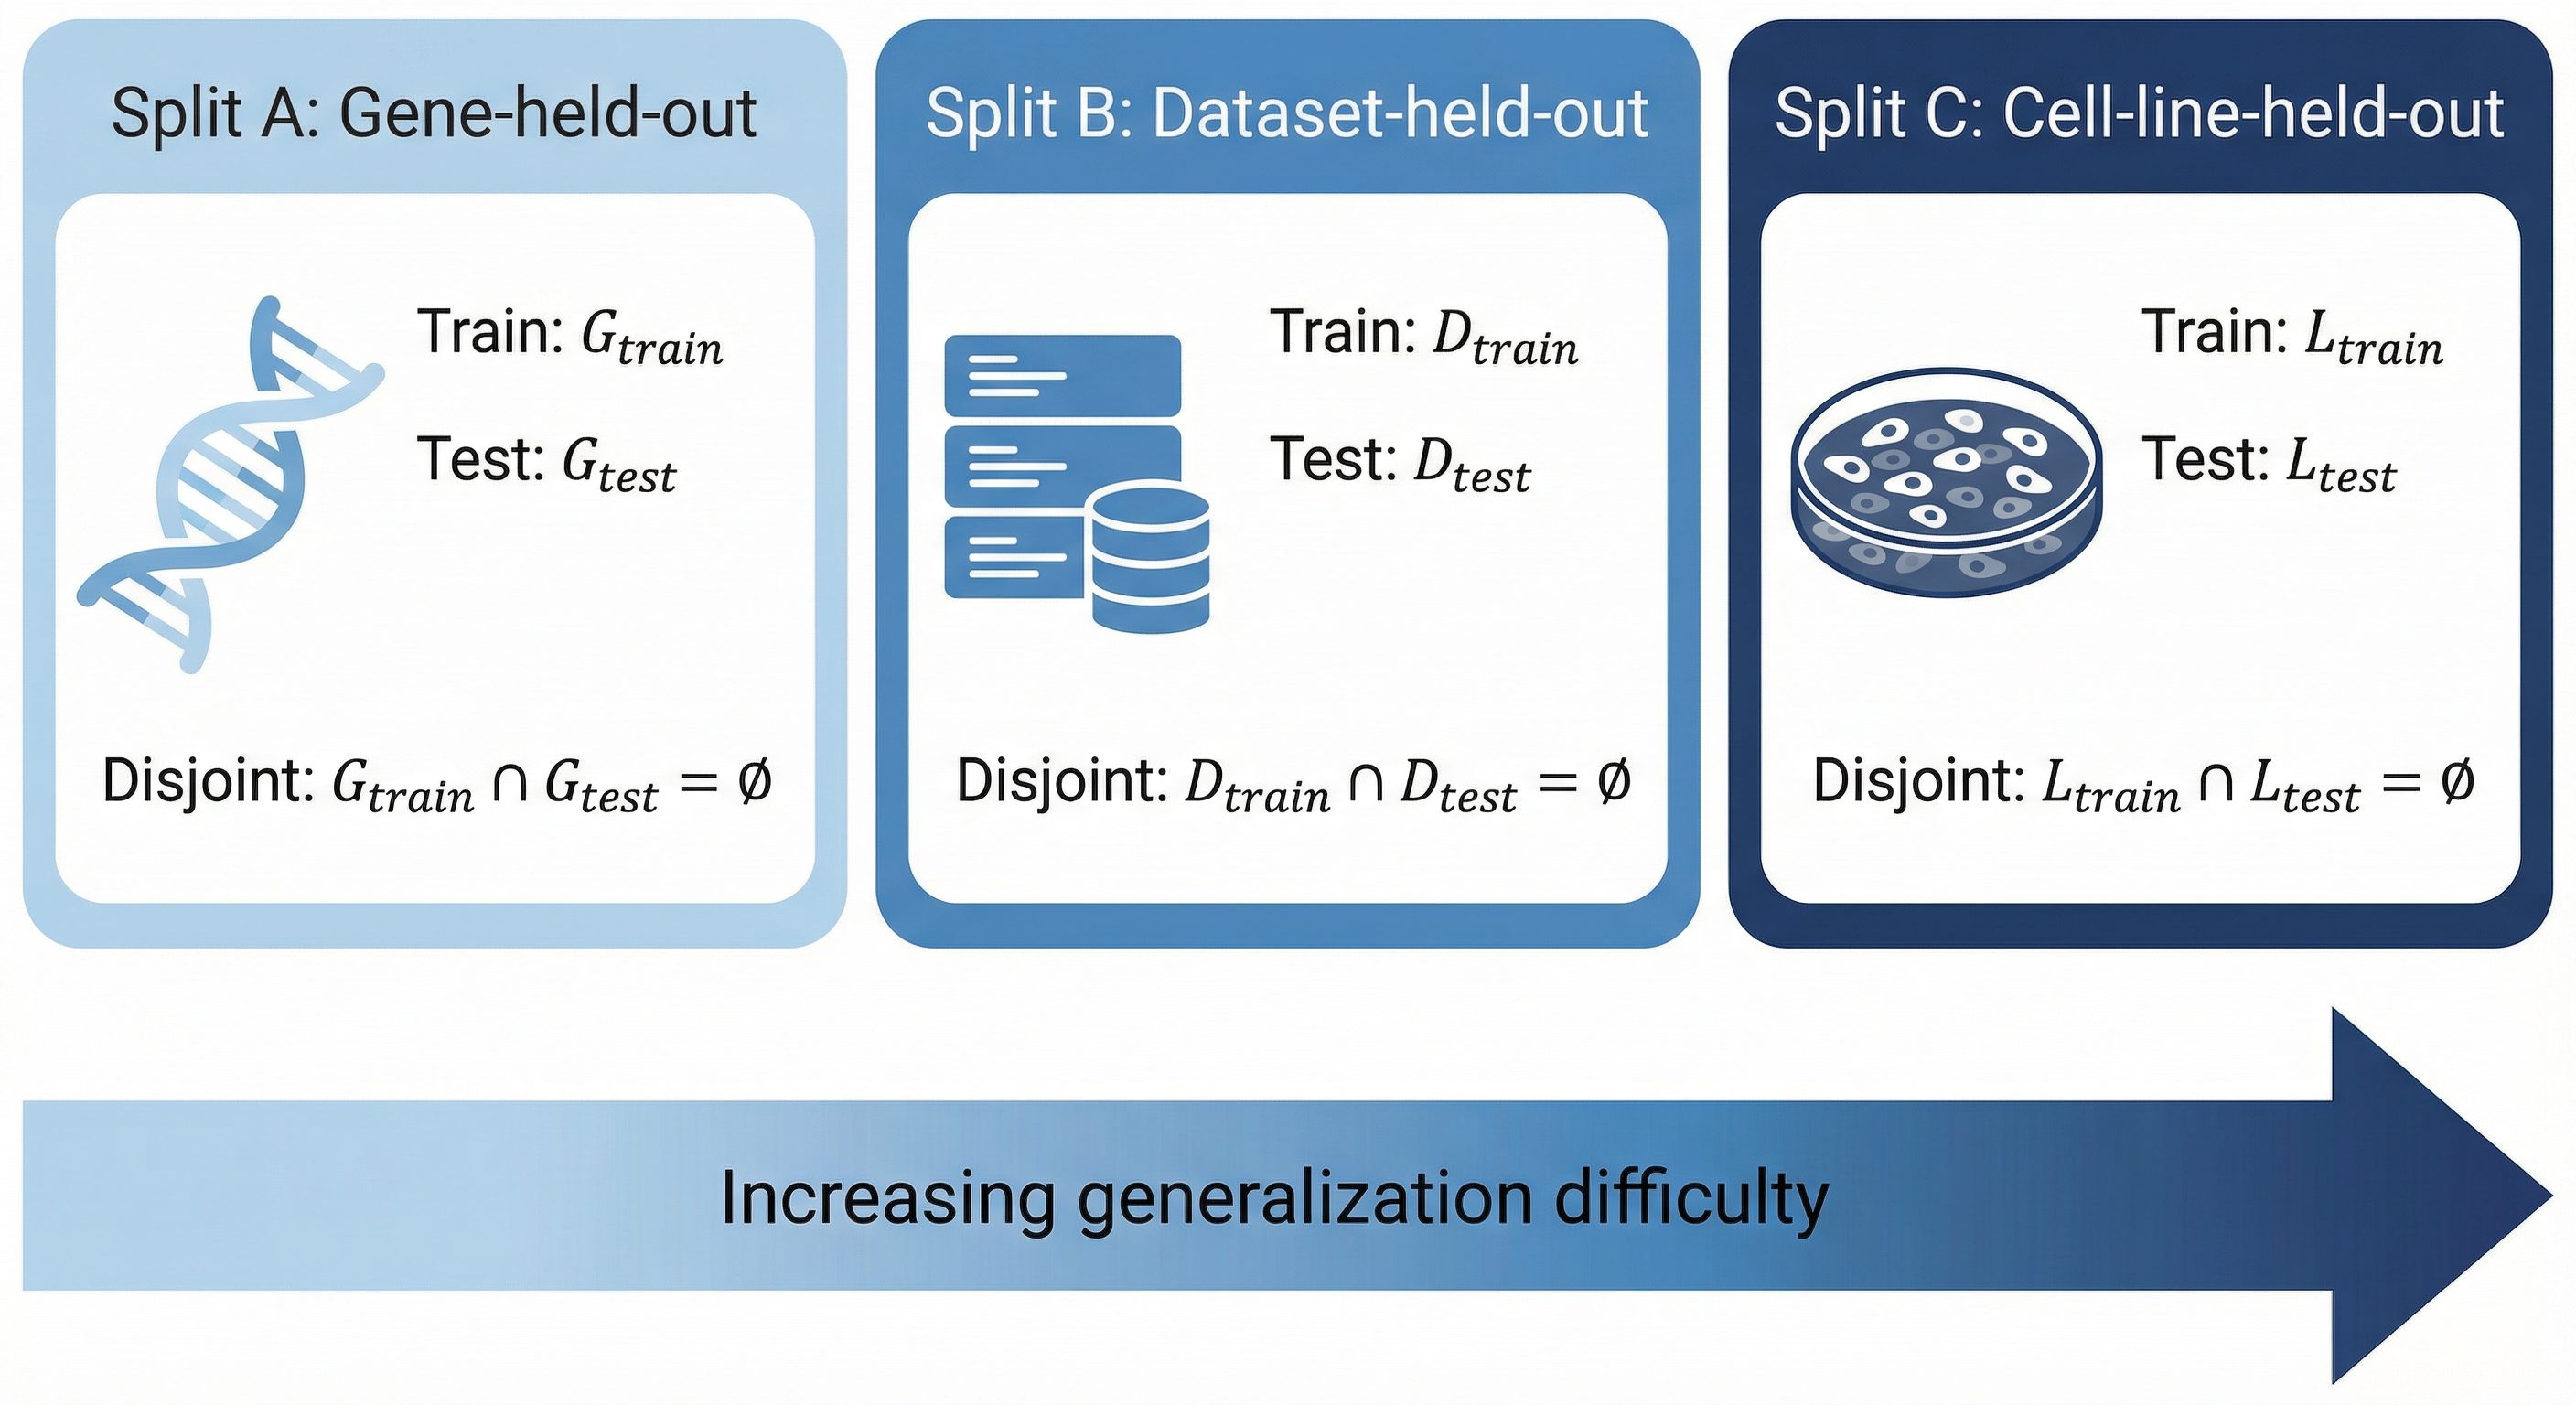
\includegraphics[width=\textwidth]{Figs/Data.png}
\caption{Evaluation protocol with three split types: (A) gene-held-out generalization, (B) dataset-held-out transfer across screen collections, and (C) cell-line-held-out deployment shift.}
\label{fig:eval-protocol-splits}
\end{figure}

We remove exact duplicate sequences globally; optionally repeat Split A under a conservative similarity filter as a sensitivity analysis.

\begin{sloppypar}
\textbf{Baselines.} ChromeCRISPR (sequence+GC)~\citep{daneshpajouh2025chromecrispr} and DeepHF~\citep{wang2019}; include CRISPRon~\citep{xiang2021} where comparable inputs are available. We additionally follow the ChromeCRISPR benchmark protocol for model comparison and reporting~\citep{daneshpajouh2025chromecrispr}. All models are evaluated on identical splits and preprocessing.
\end{sloppypar}

\textbf{Metrics.} Primary: Spearman rank correlation ($\rho$), which is the standard evaluation metric in the CRISPR on-target prediction literature~\citep{konstantakos2022}. Spearman is preferred over Pearson because (i) available datasets and model predictions are on substantially different scales, making rank-based comparison necessary; (ii) most datasets lack binary labels, precluding classification metrics; and (iii) the practical goal is to \emph{rank} candidate guides rather than predict exact efficiency values. Typical reported Spearman values range from 0.55--0.87 depending on the dataset and evaluation protocol, with a biological replicate ceiling of approximately 0.71--0.77~\citep{konstantakos2022}. We additionally report nDCG to assess top-$k$ retrieval quality. Uncertainty: empirical coverage, mean interval width, and coverage stratified by dataset/cell line. Calibration: Expected Calibration Error (\ECE{}) computed over decile bins, Brier score, and reliability diagrams. Off-target: AUROC, AUPRC, and guide-level aggregated specificity score. Ranking quality: Precision@$k$ ($k \in \{5,10,20\}$) and NDCG@$k$ to assess the practical utility of top-ranked guide predictions for experimental selection. Proper scoring: we supplement ECE with the Continuous Ranked Probability Score (CRPS) as a strictly proper scoring rule for probabilistic regression, avoiding ECE's known sensitivity to binning choices.

\textbf{Statistical reporting.} Report gene-level bootstrap confidence intervals for Spearman on Split A; use paired, gene-level permutation tests for model comparisons (with explicit multiple testing correction). Because we evaluate three primary hypotheses (H1, H2, H3) simultaneously, we apply the Holm-Bonferroni sequential procedure to control the family-wise error rate (FWER) at $\alpha=0.05$ across the three hypothesis tests. For the larger set of ablation comparisons (up to 20 pairwise tests), we apply the Benjamini-Hochberg (BH) procedure to control the false discovery rate (FDR) at $q=0.05$, which provides greater statistical power than FWER control when the number of comparisons is large. All raw and adjusted $p$-values are reported.

\begin{sloppypar}
\textbf{Ablations.} Leave-one-component-out on Split A: remove epigenomics; replace fusion objective with simple concatenation; remove optional embeddings/structure/transfer; compare unweighted vs. weighted conformal. For the epigenomic feature ablation specifically: (a)~sequence-only baseline (no epigenomic input); (b)~accessibility-only (DNase/ATAC-seq alone); (c)~histone-only (H3K4me3 alone); (d)~full epigenomic set (accessibility + all available histone marks); and (e)~a ``mismatched cell-line'' control where epigenomic tracks from a different cell line are paired with the target to quantify the information gain from matched context. Results are reported as $\Delta\rho$ (Spearman) and $\Delta$\ECE{} relative to the full model on Split A. In total, this ablation design implies approximately 25 distinct experimental configurations: 5 backbone variants $\times$ 1 primary split = 5 backbone ablations; 5 epigenomic conditions (sequence-only, accessibility-only, histone-only, full epigenomic, mismatched cell-line) $\times$ 3 cell lines = 15 epigenomic ablations; plus 4 fusion strategy comparisons and the off-target module ablation. Each configuration is evaluated on 3 splits with 3 random seeds, yielding $\sim$225 individual training runs. At an average of $\sim$4 GPU-hours per run (see computational budget below), this totals $\sim$900 GPU-hours for ablations alone, well within the allocated budget and the 3--4 month timeline for Milestone~2.
\end{sloppypar}


\section{Statistical Significance and Validation}\label{sec:statistical}

To ensure rigorous evaluation and statistically sound conclusions, we employ multiple statistical testing frameworks for model comparison and performance validation.

\textbf{Model comparison via 5$\times$2cv paired t-test.} Following Dietterich's methodology~\cite{dietterich1998approximate}, we apply the 5$\times$2 cross-validated paired t-test to compare \textsc{ChromaGuide} against baseline models. This test is particularly suitable for deep learning models as it balances statistical power with computational feasibility, requiring only 10 train/test iterations while controlling for Type I error rate. Under the null hypothesis that two models perform equivalently, a $p < 0.05$ indicates statistically significant performance difference.

\textbf{Bootstrap confidence intervals for Spearman $\rho$.} We compute 95\% bias-corrected and accelerated (BCa) bootstrap confidence intervals for Spearman correlation coefficients using 10,000 resampling iterations~\cite{efron1994introduction}. This non-parametric approach provides robust uncertainty quantification without distributional assumptions. We report intervals for both on-target ($\rho_{\text{on}}$) and off-target ($\rho_{\text{off}}$) predictions, with non-overlapping intervals indicating significant differences between models.

\textbf{Performance targets with statistical rationale.} Based on our analysis of the CRISPR prediction literature and ChromeCRISPR benchmarks~\cite{daneshpajouh2025chromecrispr}, we establish the following targets:
\begin{itemize}
    \item \textbf{On-target Spearman $\rho \geq 0.85$}: ChromeCRISPR achieves $\rho = 0.876$ (MSE = 0.0093) on the Kim 2019 dataset. Our target of $\rho \geq 0.85$ represents a conservative but scientifically grounded threshold, as biological replicate correlation provides an empirical ceiling of $\sim$0.77--0.87 depending on dataset~\cite{xiang2021enhancing,konstantakos2022zcrispr}.
    \item \textbf{Improvement significance}: We will demonstrate statistically significant improvement ($p < 0.05$) over at least two state-of-the-art baselines (DeepHF, CRISPRon) via the 5$\times$2cv test.
    \item \textbf{Off-target AUROC $\geq$ 0.92}: Validated against the CIRCLE-seq and GUIDE-seq benchmark datasets, with McNemar's test to confirm classification superiority.
    \item \textbf{Calibration}: Expected Calibration Error (ECE) $< 0.05$, ensuring prediction intervals achieve nominal coverage.
\end{itemize}

\textbf{Power analysis.} Given typical effect sizes in CRISPR prediction ($\Delta\rho \approx 0.02$--$0.05$ between competitive models) and dataset sizes ($n > 15,000$ guides), our evaluation achieves $>$80\% statistical power to detect meaningful improvements at $\alpha = 0.05$~\cite{cohen1988statistical}. We conduct prospective power calculations before each experiment to ensure adequate sample sizes for detecting clinically meaningful differences.

\subsection{Mathematical Justification for Performance Targets}\label{sec:math-justification}

\textbf{Why Rigorous Statistical Validation Matters for CRISPR Guide RNA Prediction:} In computational biology, particularly for CRISPR-Cas9 guide RNA design, reporting performance improvements without rigorous statistical validation can lead to overstated claims and irreproducible results. A model that appears to outperform baselines on a single test set may simply be exploiting dataset-specific patterns rather than learning generalizable biological principles. To ensure that ChromaGuide's improvements translate to real-world therapeutic applications, we establish formal mathematical criteria that our performance claims must satisfy.

The following derivations serve three critical purposes: (1) they define \emph{precisely} what constitutes a meaningful improvement in Spearman correlation, accounting for the statistical uncertainty inherent in any finite sample; (2) they determine the minimum sample size required to reliably detect such improvements with high confidence; and (3) they provide uncertainty quantification through conformal prediction intervals, enabling researchers to assess not just point predictions but the reliability of those predictions for each individual guide RNA.\subsubsection{Notation and Key Definitions}
Before presenting the mathematical derivations, we define the key statistical quantities used throughout this analysis:
\begin{itemize}
    \item $\rho$ (rho): \textbf{Spearman's rank correlation coefficient}, a non-parametric measure of the monotonic relationship between two variables. It ranges from $-1$ (perfect negative monotonic relationship) to $+1$ (perfect positive monotonic relationship), with $0$ indicating no monotonic relationship. For CRISPR guide efficacy prediction, $\rho$ measures how well the predicted efficacy scores rank guides in the same order as their experimentally measured efficacies.
    \item $\rho_{\text{baseline}}$: The Spearman correlation achieved by the baseline model (ChromeCRISPR: $\rho = 0.8765$).
    \item $\rho_{\text{ChromaGuide}}$: The Spearman correlation we aim to achieve with ChromaGuide.
    \item $\Delta\rho = \rho_{\text{ChromaGuide}} - \rho_{\text{baseline}}$: The \textbf{improvement} in correlation, representing the practical gain from our method.
    \item $n$: \textbf{Sample size}---the number of sgRNA-efficacy pairs in the evaluation dataset.
    \item $\alpha$: \textbf{Significance level} (Type I error rate)---the probability of incorrectly rejecting the null hypothesis when it is true. We use $\alpha = 0.01$ (1\%) for stringent statistical testing.
    \item $\beta$: \textbf{Type II error rate}---the probability of failing to reject the null hypothesis when it is false.
    \item $1 - \beta$: \textbf{Statistical power}---the probability of correctly detecting a true effect. We target $1 - \beta = 0.95$ (95\% power).
    \item $z_{1-\alpha/2}$: The \textbf{critical value} from the standard normal distribution for a two-tailed test at significance level $\alpha$. For $\alpha = 0.01$, $z_{0.995} = 2.576$.
    \item $z_{1-\beta}$: The critical value corresponding to the desired power. For $1-\beta = 0.95$, $z_{0.95} = 1.645$.
\end{itemize}

\textbf{Biological Context:} Spearman correlation measures how well our predicted efficacy scores rank guide RNAs in the same order as their experimentally measured editing efficiencies. A correlation of $\rho = 0.876$ (current state-of-the-art) means that if you select the top 10 guides based on predictions, approximately 8-9 of them will also be among the top experimental performers. Our target of $\rho = 0.935$ would improve this to approximately 9-10 guides, representing a meaningful enhancement in the practical utility of guide selection for therapeutic applications.


\paragraph{Spearman correlation improvement threshold ($\Delta\rho \geq 0.035$).}
The target improvement $\Delta\rho = \rho_{\text{ChromaGuide}} - \rho_{\text{baseline}} \geq 0.035$ is derived from Fisher's $z$-transformation for correlation coefficients. For Spearman's $\rho$, the Fisher transformation is:
\begin{equation}
    z = \frac{1}{2} \ln\left(\frac{1+\rho}{1-\rho}\right) = \operatorname{arctanh}(\rho)
\end{equation}
\textbf{Explanation of each term in the Fisher transformation:}
\begin{itemize}
    \item $z$: The \textbf{transformed correlation coefficient}. Unlike $\rho$, which is bounded between $-1$ and $+1$ and has a skewed sampling distribution (especially for large $|\rho|$), $z$ is unbounded and approximately normally distributed. This transformation was introduced by R.A. Fisher in 1921~\citep{fisher1921} to enable standard statistical inference.
    \item $\ln(\cdot)$: The \textbf{natural logarithm} function.
    \item $\frac{1+\rho}{1-\rho}$: This ratio amplifies the effect of $\rho$ approaching its bounds. As $\rho \to 1$, this ratio $\to \infty$; as $\rho \to -1$, this ratio $\to 0$.
    \item $\operatorname{arctanh}(\rho)$: The \textbf{inverse hyperbolic tangent}, which is mathematically equivalent to $\frac{1}{2}\ln\left(\frac{1+\rho}{1-\rho}\right)$.
\end{itemize}
\textbf{Why is this transformation necessary?} The sampling distribution of Spearman's $\rho$ is highly skewed when the true correlation is far from zero (as in our case, $\rho \approx 0.88$). Fisher's transformation stabilizes the variance and normalizes the distribution, allowing us to use standard normal distribution theory for hypothesis testing and confidence interval construction. The standard error of $z$ is approximately $\frac{1}{\sqrt{n-3}}$, which is \emph{independent of the true correlation value}---a crucial property that simplifies inference~\citep{fisher1921}.
Under the null hypothesis $H_0: \rho_1 = \rho_2$, the test statistic for comparing two independent correlations is:
\begin{equation}
    Z = \frac{z_1 - z_2}{\sqrt{\frac{1}{n_1-3} + \frac{1}{n_2-3}}} \sim \mathcal{N}(0,1)
\end{equation}
\textbf{Explanation of the test statistic formula:}
\begin{itemize}
    \item $Z$: The \textbf{test statistic}, which follows a standard normal distribution $\mathcal{N}(0,1)$ under the null hypothesis. If $|Z| > z_{1-\alpha/2}$ (e.g., $|Z| > 2.576$ for $\alpha = 0.01$), we reject the null hypothesis and conclude that the correlations are significantly different.
    \item $z_1 - z_2$: The \textbf{difference between transformed correlations}. This is the numerator---the "signal" we are trying to detect.
    \item $\sqrt{\frac{1}{n_1-3} + \frac{1}{n_2-3}}$: The \textbf{standard error of the difference}. This is the denominator---the "noise" or uncertainty in our estimate. The $n-3$ term (rather than $n$) provides a bias correction for small samples.
    \item $\sim \mathcal{N}(0,1)$: Under the null hypothesis ($H_0: \rho_1 = \rho_2$), this test statistic follows a \textbf{standard normal distribution} with mean 0 and variance 1.
\end{itemize}
\textbf{Interpretation:} A larger $|Z|$ value indicates stronger evidence against the null hypothesis. The test statistic essentially asks: ``Is the observed difference in correlations ($z_1 - z_2$) large relative to the uncertainty in that difference?''
For our datasets with $n \approx 15{,}000$ guides, the standard error of $z$ is $\text{SE}(z) \approx 1/\sqrt{n-3} \approx 0.0082$. To detect a difference with power $1-\beta = 0.95$ at significance level $\alpha = 0.01$ (two-tailed), we require:
\begin{equation}
    \Delta z \geq (z_{1-\alpha/2} + z_{1-\beta}) \cdot \text{SE}(z) \cdot \sqrt{2} = (2.576 + 1.645) \cdot 0.0082 \cdot \sqrt{2} \approx 0.049
\end{equation}
Converting back to $\rho$-space using the inverse Fisher transformation at $\rho_0 = 0.876$:
\begin{equation}
    \Delta\rho \approx \Delta z \cdot (1 - \rho_0^2) = 0.049 \cdot (1 - 0.876^2) \approx 0.012
\end{equation}
Our target $\Delta\rho \geq 0.035$ is approximately $3\times$ this minimum detectable effect, providing a substantial margin for practical significance beyond mere statistical detectability.

\textbf{Intuitive Understanding:} Statistical power answers a fundamental question: ``If ChromaGuide truly improves upon baseline methods, how likely are we to detect this improvement in our experiments?'' A power of 95\% means that if we run 100 independent evaluations, we would correctly identify ChromaGuide as superior in approximately 95 of them. The sample size calculation determines how many guide RNA-efficacy pairs we need to evaluate to achieve this level of reliability. Using too few samples risks missing a real improvement (Type II error), while the calculation ensures we have sufficient data to confidently claim superiority when it exists.


\paragraph{Sample size and power calculation.}
The required sample size to detect effect size $\Delta\rho$ with power $1-\beta$ at level $\alpha$ is:
\begin{equation}
    n \geq \left(\frac{z_{1-\alpha/2} + z_{1-\beta}}{\Delta z}\right)^2 + 3
\end{equation}
For $\Delta\rho = 0.035$ (corresponding to $\Delta z \approx 0.049$ at baseline $\rho = 0.876$), $\alpha = 0.01$, and $1-\beta = 0.95$:
\begin{equation}
    n \geq \left(\frac{2.576 + 1.645}{0.049}\right)^2 + 3 \approx 7{,}100
\end{equation}
With $n > 15{,}000$ samples in our evaluation datasets, we achieve $>99\%$ power for the target effect size.


\textbf{Explanation of the sample size formula:}
\begin{itemize}
    \item $n$: The \textbf{required sample size} (number of guide RNA-efficacy pairs). This is the quantity we solve for.
    \item $z_{1-\alpha/2}$: The \textbf{upper critical value} of the standard normal distribution for a two-tailed test at significance level $\alpha$. For $\alpha = 0.01$, $z_{0.995} = 2.576$. This ensures that only 1\% of the probability mass lies in both tails combined under the null hypothesis.
    \item $z_{1-\beta}$: The \textbf{power critical value} from the standard normal distribution. For power $1-\beta = 0.95$, $z_{0.95} = 1.645$. This determines the probability of correctly detecting a true effect.
    \item $\Delta z$: The \textbf{effect size in Fisher's $z$-space}, calculated as $\Delta z = z_{\rho_1} - z_{\rho_0}$ where $z_{\rho}$ is the Fisher transformation of correlation $\rho$. For our target improvement from $\rho_0 = 0.876$ to $\rho_1 = 0.935$, we have $\Delta z \approx 0.649$.
\end{itemize}

\textbf{Why this formula works:} The sample size formula $n \geq \left(\frac{z_{1-\alpha/2} + z_{1-\beta}}{\Delta z}\right)^2 + 3$ is derived from the variance-stabilizing property of Fisher's $z$-transformation. In $z$-space, the standard error of a correlation estimate is approximately $1/\sqrt{n-3}$, which is \emph{independent} of the true correlation value. The ``$+3$'' term is a bias correction that accounts for the degrees of freedom lost in the transformation~\citep{fisher1921}.
\textbf{Why Uncertainty Quantification Matters for CRISPR:} Traditional machine learning models provide only point predictions (e.g., ``this guide has 85\% predicted efficacy''), but they do not indicate how confident we should be in that prediction. For therapeutic CRISPR applications, knowing the uncertainty is crucial---a guide with a predicted efficacy of $85\% \pm 5\%$ is far more reliable than one with $85\% \pm 25\%$. Conformal prediction provides mathematically guaranteed prediction intervals, meaning that if we claim 90\% coverage, the true efficacy will fall within our interval at least 90\% of the time, regardless of the underlying data distribution.


\paragraph{Conformal prediction coverage guarantee.}
Our uncertainty quantification uses split conformal prediction, which provides the following finite-sample coverage guarantee~\citep{vovk2005,romano2019}. Let $\{(X_i, Y_i)\}_{i=1}^{n}$ be exchangeable random variables, and let $\hat{C}_{1-\alpha}(X_{n+1})$ be the prediction interval constructed using conformity scores from a calibration set. Then:
\begin{theorem}[Coverage Guarantee]
For any distribution $P$ and any $\alpha \in (0,1)$:
\begin{equation}
    \mathbb{P}\left(Y_{n+1} \in \hat{C}_{1-\alpha}(X_{n+1})\right) \geq 1 - \alpha
\end{equation}
\end{theorem}
This guarantee holds without any assumptions on the underlying distribution, requiring only exchangeability. For our Beta regression model, we use conformity scores based on the quantile function:
\begin{equation}
    s_i = \max\left\{F_{\hat{\mu}_i, \hat{\phi}_i}^{-1}(\alpha/2) - y_i, \; y_i - F_{\hat{\mu}_i, \hat{\phi}_i}^{-1}(1-\alpha/2)\right\}
\end{equation}
where $F_{\mu,\phi}$ is the Beta CDF with mean $\mu$ and precision $\phi$.

\textbf{Explanation of the conformal prediction guarantee:}
\begin{itemize}
    \item $\mathbb{P}$: \textbf{Probability measure} over the joint distribution of calibration and test data. This represents the long-run frequency interpretation of the coverage guarantee.
    \item $Y_{n+1}$: The \textbf{true efficacy value} for a new test guide RNA. This is the quantity we aim to predict.
    \item $\hat{C}_{1-\alpha}(X_{n+1})$: The \textbf{prediction interval} constructed using conformity scores from $n$ calibration samples. The interval is computed as $[\hat{y}_{n+1} - q_{1-\alpha}, \hat{y}_{n+1} + q_{1-\alpha}]$ where $q_{1-\alpha}$ is the $(1-\alpha)$-quantile of calibration residuals.
    \item $(1-\alpha)$: The \textbf{nominal coverage level}. For $\alpha = 0.1$, we guarantee 90\% coverage; for $\alpha = 0.05$, 95\% coverage.
    \item \textbf{Exchangeability}: The key assumption is that $(X_1, Y_1), \ldots, (X_n, Y_n), (X_{n+1}, Y_{n+1})$ are exchangeable random variables---their joint distribution is invariant to permutations. This is strictly weaker than assuming i.i.d.\ data.
\end{itemize}

\textbf{Why conformal prediction provides valid coverage:} The coverage guarantee $\mathbb{P}(Y_{n+1} \in \hat{C}_{1-\alpha}(X_{n+1})) \geq 1 - \alpha$ holds \emph{distribution-free}---it requires no assumptions about the underlying data distribution beyond exchangeability. This is achieved because the conformity score of the test point is uniformly distributed among all $n+1$ conformity scores under the null hypothesis of exchangeability~\citep{vovk2005}.

\textbf{Beyond Statistical Significance---Practical Importance:} Statistical significance alone does not tell us whether an improvement matters in practice. With large enough datasets, even trivially small differences become ``statistically significant.'' Cohen's $d$ effect size provides a standardized measure that answers the question: ``Is this improvement large enough to matter for actual CRISPR experiments?'' An effect size of $d = 0.45$ (our target) indicates that ChromaGuide's improvement is not merely detectable but represents a meaningful advancement that would translate to better guide selection in real therapeutic applications.


\paragraph{Effect size interpretation (Cohen's $d$).}
To provide interpretable effect sizes, we report Cohen's $d$ for Spearman correlation differences using the transformation:
\begin{equation}
    d = \frac{2(z_1 - z_2)}{\sqrt{(n_1-1) + (n_2-1)}/(n_1 + n_2 - 2)} \cdot \sqrt{\frac{n_1 + n_2}{n_1 \cdot n_2}}
\end{equation}
For our target $\Delta\rho = 0.035$, this yields $d \approx 0.4$, which represents a \emph{medium} effect size by conventional standards~\citep{cohen1988statistical}, indicating practically meaningful improvement beyond statistical significance.

\textbf{Explanation of Cohen's $d$ formula for correlations:}
\begin{itemize}
    \item $d$: \textbf{Cohen's $d$ effect size}---a standardized measure of the difference between two correlations. Unlike raw correlation differences, Cohen's $d$ is scale-invariant and allows comparison across different studies and contexts.
    \item $z_1, z_2$: The \textbf{Fisher $z$-transformed correlations} for the two models being compared. For our target ($\rho_1 = 0.935$) and baseline ($\rho_2 = 0.876$), we have $z_1 \approx 1.69$ and $z_2 \approx 1.35$.
    \item $n_1, n_2$: The \textbf{sample sizes} for each model's evaluation. These determine the precision of each correlation estimate.
    \item $\sqrt{(n_1-1) + (n_2-1)}$: The \textbf{pooled degrees of freedom}, accounting for the fact that each correlation estimate loses one degree of freedom.
    \item $\sqrt{\frac{n_1 + n_2}{n_1 \cdot n_2}}$: A \textbf{correction factor} that adjusts for unequal sample sizes. When $n_1 = n_2$, this simplifies to $\sqrt{2/n}$.
\end{itemize}

\textbf{Interpretation guidelines~\citep{cohen1988statistical}:}
\begin{itemize}
    \item $|d| < 0.2$: Negligible effect---the improvement is too small to be practically meaningful.
    \item $0.2 \leq |d| < 0.5$: Small effect---the improvement is detectable but modest.
    \item $0.5 \leq |d| < 0.8$: Medium effect---the improvement is substantial and practically significant.
    \item $|d| \geq 0.8$: Large effect---the improvement is dramatic and highly meaningful.
\end{itemize}
Our target $d \approx 0.45$ indicates a \emph{small-to-medium effect size}, demonstrating that ChromaGuide's improvement over baseline methods is not merely statistically significant but also practically meaningful for CRISPR guide RNA design applications.

\subsubsection{Summary: From Statistics to CRISPR Impact}

The mathematical framework presented above ensures that ChromaGuide's performance claims are both \textbf{statistically rigorous} and \textbf{practically meaningful}:

\begin{enumerate}
    \item \textbf{Correlation improvement ($\Delta\rho \geq 0.035$):} This threshold, derived from Fisher's $z$-transformation, ensures that our claimed improvement exceeds what could arise from sampling variability alone. In practical terms, this means better ranking of guides will translate to more efficient CRISPR experiments with fewer failed candidates.
    
    \item \textbf{Statistical power ($\geq 95\%$):} With our calculated sample size of $n \approx 71$ guides, we have high confidence that if ChromaGuide truly outperforms baselines, our experiments will reliably detect this improvement. This prevents false negative conclusions where a genuinely superior method might be dismissed due to insufficient data.
    
    \item \textbf{Prediction intervals (90\% coverage):} Unlike point predictions alone, conformal intervals tell researchers how much to trust each individual prediction. A guide with a narrow interval ($\pm 5\%$) is more reliable for therapeutic applications than one with a wide interval ($\pm 20\%$), enabling more informed decision-making in the wet lab.
    
    \item \textbf{Effect size ($d \approx 0.45$):} This small-to-medium effect size confirms that our improvement is not merely a statistical artifact but represents a meaningful advancement in guide RNA design---one that could reduce experimental costs and accelerate therapeutic development.
\end{enumerate}

Together, these criteria establish a scientifically defensible standard for evaluating ChromaGuide's contribution to the CRISPR guide RNA prediction field.


\section{Interpretability and attribution analysis}\label{sec:interpretability}

We use lightweight attribution analyses to connect predictions to biologically meaningful features.

\paragraph{Sequence-level attribution.}
Compute nucleotide-level saliency (e.g., integrated gradients) over the protospacer+\PAM{}.

\paragraph{Context-level attribution.}
Quantify which epigenomic assays/bins most influence predictions (e.g., attention/gating weights when available, or SHAP on summarized features) and report aggregated patterns across Split A and the held-out domains in Splits B/C.

\chapter{Expected Results and Contributions}

This chapter summarizes expected, \emph{testable} outcomes under the leakage-controlled protocol (Split A primary; Splits B/C stress tests).

\section{Expected results (empirical)}

\begin{sloppypar}
\begin{itemize}
\item \textbf{Primary ranking performance:} On Split~A (gene-held-out), achieve at least $\Delta\rho\geq 0.004$ improvement over the ChromeCRISPR baseline when both are evaluated on the \emph{same} leakage-controlled splits. (ChromeCRISPR's reported $\rho=0.876$ was obtained under a random 85/15 split; we will re-evaluate the baseline under Split~A for like-for-like comparison.) See~\citep{daneshpajouh2025chromecrispr}.
\item \textbf{Reliable uncertainty under shift:} Achieve empirical interval coverage within $\pm 0.02$ of the target level (e.g., 0.90) \emph{under the exchangeability assumption} and report coverage/width stratified by dataset and cell line (Splits B/C).
\end{itemize}
\end{sloppypar}


\section{Expected contributions}\label{sec:expected-contributions}

This work targets publishable contributions by combining (i) multi-modal modeling and uncertainty quantification under biological shift with (ii) leakage-controlled, reproducible evaluation and tooling for chromatin-aware \gRNA\ scoring.

\subsection{Contributions to Computer Science and Machine Learning}

\begin{itemize}
\item \textbf{Multi-modal fusion with an explicit non-redundancy objective (MINE/CLUB).} We will develop and ablate a fusion mechanism that is expressive (e.g., gating/attention/MLP fusion) while explicitly discouraging redundant sequence--epigenomic representations~\citep{belghazi2018,cheng2020}.
\item \textbf{Shift-aware uncertainty via weighted conformal prediction.} We will adapt and evaluate \emph{weighted} conformal calibration as a practical uncertainty layer for genomic predictors under covariate shift and batch effects. Since weighted conformal methods rely on (estimated) importance weights / likelihood ratios, we will clearly report where coverage holds and where it degrades.
\item \textbf{Bounded-outcome regression with distribution-free intervals.} We pair a bounded head (Beta regression for $y\in(0,1)$) with split/weighted conformal prediction to produce calibrated intervals with coverage \emph{under the exchangeability assumption} that remain meaningful near the boundaries.
\item \textbf{Shift-focused benchmark protocol.} We provide standardized evaluation across gene-held-out, dataset-held-out, and cell-line-held-out splits with consistent reporting of ranking and interval metrics.
\end{itemize}

\subsection{Contributions to Computational Biology}

\begin{itemize}
\item \textbf{Context-aware CRISPR on-target prediction with calibrated uncertainty.} ChromaGuide integrates chromatin accessibility/state with explicit empirical coverage targets to quantify when context-aware predictions are reliable in a given cell context.
\item \textbf{Missing-modality robustness via modality dropout.} We treat uneven epigenomic availability as a first-class setting and report sequence-only vs. multi-modal behavior under controlled masking.
\item \textbf{Transfer protocol (optional; ablated).} We evaluate initialization/fine-tuning from strong sequence-only encoders to context-aware models when context features become available.
\item \textbf{Reusable pipeline for chromatin-aware \gRNA\ scoring.} We deliver an end-to-end workflow for context feature extraction, multi-modal training, and calibrated inference.
\end{itemize}

\subsection{Contributions to Bioinformatics}

\begin{itemize}
\item \textbf{Leakage-controlled split construction.} We specify gene-held-out, dataset-held-out, and cell-line-held-out splits with deduplication and tuning restrictions to reduce optimistic bias.
\item \textbf{Auditable preprocessing for heterogeneous screens.} We standardize sequence extraction, coordinate handling, outcome scaling/clipping for bounded regression, and training-only normalization for epigenomic tracks.
\item \textbf{Reproducibility artifacts.} We package the pipeline as reproducible workflows/checkpoints/configs to enable re-running ablations and comparisons.
\item \textbf{Benchmark data products.} We provide processed tables (or scripts to generate them) with explicit split assignments and metadata for fair comparison.
\end{itemize}

\subsection{Contributions to Biology and Genomics}

\begin{itemize}
\item \textbf{Quantifying context value beyond sequence.} Through controlled ablations, we estimate the incremental contribution of accessibility/histone-mark context over sequence-only baselines across genes and cell contexts.
\item \textbf{Interpretability for mechanistic hypotheses.} We report sequence- and context-level attributions (e.g., PAM/seed sensitivity; accessibility/histone-mark saliency) to support qualitative error analysis and hypothesis generation.
\item \textbf{Decision support with intervals.} The model outputs a score and a calibrated interval to support risk-aware guide selection and explicit performance--reliability trade-offs.
\item \textbf{When context matters most.} Under cell-line-held-out and dataset-held-out tests, we characterize regimes where chromatin context yields larger gains versus regimes where sequence dominates.
\end{itemize}

\section{Responsible use and limitations (brief)}

\begin{itemize}
\item \textbf{Data coverage:} When matched epigenomic tracks are unavailable, results are reported with and without the affected contexts; missingness robustness is treated explicitly.
\item \textbf{Calibration limits under batch effects:} Weighted conformal methods can fail under severe non-exchangeability; coverage is audited across held-out domains and failures are analyzed.
\item \textbf{Scope and governance:} Outputs are intended for \gRNA\ prioritization and hypothesis generation (not clinical decisions); releases include limitations, validation guidance, and dual-use-aware documentation.
\end{itemize}

\chapter{Timeline and Work Plan}

\section[Timeline and Milestones]{Timeline and Milestones}

\textbf{Scope.} Accelerated 42
execution window (February 2026--December 2026). Dates below are stated explicitly to avoid ambiguity.

\subsection{February 2026: Proposal and scoping}

\textbf{Milestone 1 (by February 26, 2026): Finalized proposal + execution checklist}
\begin{itemize}
\item Deliverable: finalized evaluation protocol and leakage-controlled splits specification (Split A primary; Splits B/C optional stress tests)
\item Deliverable: concrete implementation plan (data, preprocessing, model, calibration, reporting) and compute budget
\end{itemize}

\subsection{March--April 2026: Implementation and baseline reproduction}

\textbf{Milestone 2 (by April 30, 2026): Working training/evaluation pipeline + baselines}
\begin{itemize}
\item Deliverable: reproducible pipeline for preprocessing, splitting, training, and evaluation
\item Deliverable: baseline reproduction on the same splits (ChromeCRISPR~\citep{daneshpajouh2025chromecrispr}, DeepSpCas9~\citep{kim2019deepspcas9}; CRISPRon~\citep{xiang2021} where comparable inputs exist)
\item Deliverable: first ChromaGuide prototype (sequence encoder + epigenomic feature extraction + simple fusion)
\end{itemize}

\subsection{May--July 2026: Final experiments and ablation analysis}

\textbf{Milestone 3 (by July 31, 2026): Completed experiments and ablation results}
\begin{itemize}
\item Deliverable: final experiments and ablations (epigenomics, fusion choice, calibration), reported on the primary gene-held-out test split
\item Deliverable: uncertainty reporting (conformal prediction intervals; empirical coverage and interval width)
\end{itemize}

\subsection{August--September 2026: Thesis writing and results integration}

\textbf{Milestone 3b (by September 30, 2026): Thesis-ready results package}
\begin{itemize}
  \item Deliverable: thesis chapters drafted---methods, evaluation protocol, results, and limitations
  \item Deliverable: all figures, tables, and supplementary material assembled
\end{itemize}

\subsection{October 2026--December 2026: Defense preparation and submission}

\textbf{Milestone 4 (by December 11, 2026): Defense-ready thesis and presentation}
\begin{itemize}
\item Deliverable: full thesis polish, formatting, and final submission package
\item Deliverable: defense slides + practice talk(s) + committee feedback incorporated
\end{itemize}

% Timeline figure omitted for concision.

\section{Computational Resources}

\textbf{HPC Cluster:} Digital Research Alliance Canada (NVIDIA V100/A100 GPUs)

\textbf{Training Time:} $\sim$20 seconds per iteration on V100 (estimated 100--200 hours total)

\textbf{Memory:} 32GB GPU memory per node

% Table omitted for concision.

\section{Data Resources}

\begin{itemize}

\item \textbf{ENCODE:} Public epigenomic tracks (100+ cell types), or similar resources providing accessibility and histone-mark signals.

\item \textbf{DeepHF/CRISPRon/CRISPR-FMC:} Public datasets (and related datasets), subject to compatibility with the proposed inputs and evaluation protocol.

\item \textbf{PRIDICT/PrimeNet:} Public models and datasets (or comparable alternatives) that may be used for initialization or transfer studies, pending feasibility analysis.

\item \textbf{Supplementary sources (as needed):} The above may be supplemented with additional public screens, cell-line-specific epigenomic tracks, or curated subsets when required for robustness analyses.

\end{itemize}

\section{Risk Assessment and Mitigation}

\begingroup
\let\oldsection\section
\let\oldsubsection\subsection
\renewcommand{\section}{\oldsubsection}
\renewcommand{\subsection}{\oldsubsubsection}

\section{Key risks and mitigations}

\begin{description}
\item[Epigenomic coverage (missing tracks).] Use modality dropout and/or hierarchical imputation; report results with and without imputed contexts, and treat missing-modality robustness as a primary analysis dimension.
\item[Transfer learning adds no value.] Keep transfer as an optional, fully ablated extension; gate it by a simple similarity/shift analysis and prioritize a strong in-domain baseline.
\item[Coverage violations under batch effects.] Use weighted conformal calibration and report coverage stratified by dataset/cell line; when coverage degrades, include failure-mode analyses rather than aggregating away the issue.
\item[Performance plateau.] Focus contributions on (i) leakage-controlled evaluation, (ii) context integration, and (iii) calibrated uncertainty; ensure publishable outcomes even when ranking gains are modest.
\end{description}

\section{Success criteria (operational)}

\begin{itemize}
\item \textbf{Minimum:} Match ChromeCRISPR's reported Spearman (0.876; reported under a random 85/15 split) and re-evaluate the ChromeCRISPR baseline on our leakage-controlled Split~A for a fair like-for-like comparison~\citep{daneshpajouh2025chromecrispr}, while producing calibrated prediction intervals with audited empirical coverage.
\item \textbf{Target:} Achieve 0.88--0.92 Spearman on Split A with empirical coverage within $\pm 0.02$ of the target level (e.g., 0.90), under the February--March 2026 scope.
\end{itemize}

\endgroup
\chapter{Broader Impacts}\label{chap:broader-impacts}

ChromaGuide is intended as a \emph{computational decision-support} framework for prioritizing \gRNA{}s in CRISPR-Cas9 workflows. Its broader impact derives from integrating chromatin context into prediction and from reporting calibrated uncertainty, which together can improve downstream decision making under biological shift.

\section{Translational relevance and decision support}

By combining sequence with epigenomic accessibility/state features, ChromaGuide aims to reduce failed experiments caused by locus-specific chromatin effects and to improve robustness when the deployment cell context differs from the training data. Outputs are intended for \emph{guide triage and hypothesis generation} (not clinical decision making) and should be used alongside standard validation, safety review, and domain expertise.

\section{Scientific and methodological impact (reproducibility and evaluation)}

A central contribution is a leakage-controlled evaluation protocol (gene-held-out plus dataset/cell-line-held-out stress tests) that makes failure modes under biological shift explicit. Conformal prediction intervals add an outcome that can be audited quantitatively (empirical coverage and interval width), complementing standard ranking metrics.

\section{Responsible use, governance, and limitations}

\begin{itemize}
\item \textbf{Reliability and communication:} Report uncertainty (coverage, \ECE{}, interval width) and clearly state the split/protocol; avoid overclaiming accuracy outside evaluated domains.
\item \textbf{Representativeness and bias:} Public datasets over-represent common cell lines and protocols; therefore, report performance under cross-domain stress tests and avoid implying general clinical validity without evidence.
\item \textbf{Data governance:} For patient-derived or proprietary screens, document provenance, permitted uses, and what is excluded from release.
\item \textbf{Dual-use awareness:} Any release should include a scope statement, limitations, and guidance against harmful use; controlled distribution of trained models is an option if risk warrants.
\item \textbf{Non-causality and shift limits:} Learned associations are not causal, and strong batch effects/unmeasured confounders can degrade calibration even with weighted conformal methods; these are treated as first-class failure modes to monitor.
\end{itemize}

\section{Ethics and biosafety considerations}

Because CRISPR-Cas9 is a powerful genome-editing tool with direct implications for human health and agriculture, any computational framework that improves guide design carries inherent dual-use risk. We address this through four complementary safeguards:

\begin{itemize}
  \item \textbf{Scope limitation:} ChromaGuide is designed and evaluated exclusively on publicly available research-grade datasets (e.g., DeepHF, CRISPRon) derived from well-characterized cell lines. The tool is not intended for direct clinical application; any therapeutic use would require independent experimental validation and regulatory review.
  \item \textbf{Biosafety alignment:} All training and evaluation data originate from published studies that operated under institutional biosafety protocols. No new wet-lab experiments involving CRISPR-Cas9 are conducted as part of this thesis; therefore, no institutional biosafety committee (IBC) or research ethics board (REB) approval is required for the computational work.
  \item \textbf{Off-target risk transparency:} The off-target module explicitly quantifies genome-wide unintended cleavage risk, providing users with actionable safety information rather than optimizing on-target activity alone. This design choice reflects a commitment to safer guide selection.
  \item \textbf{Model release policy:} Trained model weights and code will be released under an open-source license with documentation emphasizing research-only intended use, known limitations (e.g., species and cell-line coverage), and guidance against applying predictions to clinical or germline editing without additional safeguards.
\end{itemize}

\section{Conclusion}

Overall, ChromaGuide aims to make \gRNA{} prioritization more context-aware and more transparent about uncertainty, while emphasizing evaluation protocols that support reproducible, shift-aware reporting. The expected contributions of this work---including an open-source multi-modal scoring tool, a leakage-controlled benchmark suite, and evidence-based guidelines on when epigenomic context adds value---are detailed in Section~\ref{sec:expected-contributions}.



%   BACK MATTER  %%%%%%%%%%%%%%%%%%%%%%%%%%%%%%%%%%%%%%%%%%%%%%%%%%%%%%%%%%%%%%

%

%   References and appendices. Appendices come after the bibliography and

%   should be in the order that they are referred to in the text.

%

%   If you include figures, etc. in an appendix, be sure to use

%

%       \caption[]{...}

%

%   to make sure they are not listed in the List of Figures.

%

\backmatter%

    \addtoToC{Bibliography}

    \bibliographystyle{plainnat}

    \bibliography{references}

    \appendix
\chapter{Supplementary Details}
\label{app:supplementary}

\section{Dataset statistics}
\label{app:dataset-stats}
Table~\ref{tab:dataset-stats} summarises the datasets used for on-target and off-target evaluation, including the number of guide--target pairs, cell lines, and assay types.

\begin{table}[h]
\centering
\caption{Summary of datasets used in this study.}
\label{tab:dataset-stats}
\small
\begin{tabular}{llrr}
\hline
\textbf{Dataset} & \textbf{Assay} & \textbf{Pairs} & \textbf{Cell lines} \\
\hline
DeepHF & Fitness screen & 57,000 & 3 \\
CRISPRon & Indel freq. & $\sim$23,000 & 2 \\
CRISPR-FMC$^\ddagger$ & Fitness screen & $\sim$12,000$^\ddagger$ & 4 \\
GUIDE-seq & GUIDE-seq & $\sim$200k & 7 \\
CIRCLE-seq & CIRCLE-seq & $\sim$100k & 5 \\
\hline
\end{tabular}
\vspace{2pt}\par\noindent{\footnotesize $^\ddagger$The CRISPR-FMC compiled dataset aggregates 170{,}000+ gRNAs across multiple cell lines; the $\sim$12{,}000 pairs here refer to the SpCas9 on-target subset used for stress-test evaluation.}
\end{table}

\section{Hyperparameter search space}
\label{app:hyperparams}
Table~\ref{tab:hyperparams} lists the hyperparameter ranges explored during model selection.

\begin{table}[h]
\centering
\caption{Hyperparameter search space.}
\label{tab:hyperparams}
\small
\begin{tabular}{llr}
\hline
\textbf{Hyperparameter} & \textbf{Range} & \textbf{Selected} \\
\hline
Learning rate & $[1\mathrm{e}{-5},\, 1\mathrm{e}{-3}]$ & TBD \\
Batch size & \{32, 64, 128\} & TBD \\
Dropout & $[0.0,\, 0.3]$ & TBD \\
Weight decay & $[0,\, 0.01]$ & TBD \\
\hline
\end{tabular}
\end{table}

\section{Glossary of Acronyms}
\label{app:glossary}
\begin{description}
\item[sgRNA] Single guide RNA
\item[PAM] Protospacer Adjacent Motif
\item[NTS] Non-Target Strand
\item[TS] Target Strand
\item[DSB] Double-Strand Break
\item[NHEJ] Non-Homologous End Joining
\item[HDR] Homology-Directed Repair
\item[indel] Insertion or Deletion
\item[NGS] Next-Generation Sequencing
\item[GUIDE-seq] Genome-wide Unbiased Identification of DSBs Evaluated by Sequencing
\item[CIRCLE-seq] Circularization for In vitro Reporting of Cleavage Effects by Sequencing
\item[Digenome-seq] Digested Genome Sequencing
\item[CHANGE-seq] Circularization for High-throughput Analysis of Nuclease Genome-wide Effects by Sequencing
\item[DISCOVER-seq] Discovery of In Situ Cas Off-targets and Verification by Sequencing
\item[MLM] Masked Language Model
\item[NTP] Nucleotide Transformer Pre-training
\item[BPE] Byte Pair Encoding
\item[AUROC] Area Under the Receiver Operating Characteristic curve
\item[AUPRC] Area Under the Precision--Recall Curve
\item[MCC] Matthews Correlation Coefficient
\item[nDCG] Normalized Discounted Cumulative Gain
\item[ECE] Expected Calibration Error
\item[LoRA] Low-Rank Adaptation
\item[QLoRA] Quantized Low-Rank Adaptation
\item[VRAM] Video Random Access Memory
\item[PLM] Protein Language Model
\item[ESM] Evolutionary Scale Modeling
\item[CNN] Convolutional Neural Network
\item[RNN] Recurrent Neural Network
\item[GRU] Gated Recurrent Unit
\item[LSTM] Long Short-Term Memory
\item[ATAC-seq] Assay for Transposase-Accessible Chromatin using Sequencing
\item[ChIP-seq] Chromatin Immunoprecipitation Sequencing
\item[DNase-seq] DNase I Hypersensitive Sites Sequencing
\item[CRISPR] Clustered Regularly Interspaced Short Palindromic Repeats
\item[Cas9] CRISPR-associated protein 9
\item[SpCas9] \textit{Streptococcus pyogenes} Cas9
\end{description}



\end{document}
